\documentclass[twoside]{book}

% Packages required by doxygen
\usepackage{fixltx2e}
\usepackage{calc}
\usepackage{doxygen}
\usepackage{graphicx}
\usepackage[utf8]{inputenc}
\usepackage{makeidx}
\usepackage{multicol}
\usepackage{multirow}
\PassOptionsToPackage{warn}{textcomp}
\usepackage{textcomp}
\usepackage[nointegrals]{wasysym}
\usepackage[table]{xcolor}

% NLS support packages
\usepackage[french]{babel}

% Font selection
\usepackage[T1]{fontenc}
\usepackage{mathptmx}
\usepackage[scaled=.90]{helvet}
\usepackage{courier}
\usepackage{amssymb}
\usepackage{sectsty}
\renewcommand{\familydefault}{\sfdefault}
\allsectionsfont{%
  \fontseries{bc}\selectfont%
  \color{darkgray}%
}
\renewcommand{\DoxyLabelFont}{%
  \fontseries{bc}\selectfont%
  \color{darkgray}%
}
\newcommand{\+}{\discretionary{\mbox{\scriptsize$\hookleftarrow$}}{}{}}

% Page & text layout
\usepackage{geometry}
\geometry{%
  a4paper,%
  top=2.5cm,%
  bottom=2.5cm,%
  left=2.5cm,%
  right=2.5cm%
}
\tolerance=750
\hfuzz=15pt
\hbadness=750
\setlength{\emergencystretch}{15pt}
\setlength{\parindent}{0cm}
\setlength{\parskip}{0.2cm}
\makeatletter
\renewcommand{\paragraph}{%
  \@startsection{paragraph}{4}{0ex}{-1.0ex}{1.0ex}{%
    \normalfont\normalsize\bfseries\SS@parafont%
  }%
}
\renewcommand{\subparagraph}{%
  \@startsection{subparagraph}{5}{0ex}{-1.0ex}{1.0ex}{%
    \normalfont\normalsize\bfseries\SS@subparafont%
  }%
}
\makeatother

% Headers & footers
\usepackage{fancyhdr}
\pagestyle{fancyplain}
\fancyhead[LE]{\fancyplain{}{\bfseries\thepage}}
\fancyhead[CE]{\fancyplain{}{}}
\fancyhead[RE]{\fancyplain{}{\bfseries\leftmark}}
\fancyhead[LO]{\fancyplain{}{\bfseries\rightmark}}
\fancyhead[CO]{\fancyplain{}{}}
\fancyhead[RO]{\fancyplain{}{\bfseries\thepage}}
\fancyfoot[LE]{\fancyplain{}{}}
\fancyfoot[CE]{\fancyplain{}{}}
\fancyfoot[RE]{\fancyplain{}{\bfseries\scriptsize Généré le Dimanche 17 Mai 2015 19\+:48\+:56 pour Visualiseur d'algorithme par Doxygen }}
\fancyfoot[LO]{\fancyplain{}{\bfseries\scriptsize Généré le Dimanche 17 Mai 2015 19\+:48\+:56 pour Visualiseur d'algorithme par Doxygen }}
\fancyfoot[CO]{\fancyplain{}{}}
\fancyfoot[RO]{\fancyplain{}{}}
\renewcommand{\footrulewidth}{0.4pt}
\renewcommand{\chaptermark}[1]{%
  \markboth{#1}{}%
}
\renewcommand{\sectionmark}[1]{%
  \markright{\thesection\ #1}%
}

% Indices & bibliography
\usepackage{natbib}
\usepackage[titles]{tocloft}
\setcounter{tocdepth}{3}
\setcounter{secnumdepth}{5}
\makeindex

% Hyperlinks (required, but should be loaded last)
\usepackage{ifpdf}
\ifpdf
  \usepackage[pdftex,pagebackref=true]{hyperref}
\else
  \usepackage[ps2pdf,pagebackref=true]{hyperref}
\fi
\hypersetup{%
  colorlinks=true,%
  linkcolor=blue,%
  citecolor=blue,%
  unicode%
}

% Custom commands
\newcommand{\clearemptydoublepage}{%
  \newpage{\pagestyle{empty}\cleardoublepage}%
}


%===== C O N T E N T S =====

\begin{document}

% Titlepage & ToC
\hypersetup{pageanchor=false,
             bookmarks=true,
             bookmarksnumbered=true,
             pdfencoding=unicode
            }
\pagenumbering{roman}
\begin{titlepage}
\vspace*{7cm}
\begin{center}%
{\Large Visualiseur d'algorithme }\\
\vspace*{1cm}
{\large Généré par Doxygen 1.8.8}\\
\vspace*{0.5cm}
{\small Dimanche 17 Mai 2015 19:48:56}\\
\end{center}
\end{titlepage}
\clearemptydoublepage
\tableofcontents
\clearemptydoublepage
\pagenumbering{arabic}
\hypersetup{pageanchor=true}

%--- Begin generated contents ---
\chapter{Index hiérarchique}
\section{Hiérarchie des classes}
Cette liste d'héritage est classée approximativement par ordre alphabétique \+:\begin{DoxyCompactList}
\item \contentsline{section}{cellule}{\pageref{structcellule}}{}
\item \contentsline{section}{File}{\pageref{classFile}}{}
\item \contentsline{section}{Liste}{\pageref{classListe}}{}
\item \contentsline{section}{liste\+\_\+adjacence\+\_\+t}{\pageref{structliste__adjacence__t}}{}
\item \contentsline{section}{matrice\+\_\+adjacence\+\_\+t}{\pageref{structmatrice__adjacence__t}}{}
\item \contentsline{section}{matrice\+\_\+laplace\+\_\+t}{\pageref{structmatrice__laplace__t}}{}
\item \contentsline{section}{parcours\+\_\+t}{\pageref{structparcours__t}}{}
\item Q\+Main\+Window\begin{DoxyCompactList}
\item \contentsline{section}{Main\+Window}{\pageref{classMainWindow}}{}
\end{DoxyCompactList}
\item Q\+Open\+G\+L\+Widget\begin{DoxyCompactList}
\item \contentsline{section}{Scene\+G\+L}{\pageref{classSceneGL}}{}
\end{DoxyCompactList}
\item \contentsline{section}{Scene\+Vertex}{\pageref{structSceneVertex}}{}
\item \contentsline{section}{Shader}{\pageref{classShader}}{}
\item \contentsline{section}{sommet}{\pageref{structsommet}}{}
\item \contentsline{section}{Structure}{\pageref{classStructure}}{}
\begin{DoxyCompactList}
\item \contentsline{section}{Graphe}{\pageref{classGraphe}}{}
\end{DoxyCompactList}
\end{DoxyCompactList}

\chapter{Index des classes}
\section{Liste des classes}
Liste des classes, structures, unions et interfaces avec une brève description \+:\begin{DoxyCompactList}
\item\contentsline{section}{\hyperlink{structcellule}{cellule} }{\pageref{structcellule}}{}
\item\contentsline{section}{\hyperlink{classFile}{File} }{\pageref{classFile}}{}
\item\contentsline{section}{\hyperlink{classGraphe}{Graphe} \\*Classe gerant la structure de donnée de graphe }{\pageref{classGraphe}}{}
\item\contentsline{section}{\hyperlink{classListe}{Liste} }{\pageref{classListe}}{}
\item\contentsline{section}{\hyperlink{structliste__adjacence__t}{liste\+\_\+adjacence\+\_\+t} }{\pageref{structliste__adjacence__t}}{}
\item\contentsline{section}{\hyperlink{classMainWindow}{Main\+Window} \\*Classe gerant le placement et interactions des principaux widgets dans la fenetre principale }{\pageref{classMainWindow}}{}
\item\contentsline{section}{\hyperlink{structmatrice__adjacence__t}{matrice\+\_\+adjacence\+\_\+t} }{\pageref{structmatrice__adjacence__t}}{}
\item\contentsline{section}{\hyperlink{structmatrice__laplace__t}{matrice\+\_\+laplace\+\_\+t} }{\pageref{structmatrice__laplace__t}}{}
\item\contentsline{section}{\hyperlink{structparcours__t}{parcours\+\_\+t} }{\pageref{structparcours__t}}{}
\item\contentsline{section}{\hyperlink{classSceneGL}{Scene\+G\+L} \\*Classe gerant le contexte Open\+G\+L de l'application }{\pageref{classSceneGL}}{}
\item\contentsline{section}{\hyperlink{structSceneVertex}{Scene\+Vertex} \\*\hyperlink{classStructure}{Structure} d'un vertex incluant sa position et couleur }{\pageref{structSceneVertex}}{}
\item\contentsline{section}{\hyperlink{classShader}{Shader} \\*Classe gerant la compilation et verrouillage du vertex et fragment shaders }{\pageref{classShader}}{}
\item\contentsline{section}{\hyperlink{structsommet}{sommet} }{\pageref{structsommet}}{}
\item\contentsline{section}{\hyperlink{classStructure}{Structure} \\*Classe gerant les structures de données chargées dans l'I\+H\+M }{\pageref{classStructure}}{}
\end{DoxyCompactList}

\chapter{Index des fichiers}
\section{Liste des fichiers}
Liste de tous les fichiers documentés avec une brève description \+:\begin{DoxyCompactList}
\item\contentsline{section}{{\bfseries cellule.\+cpp} }{\pageref{cellule_8cpp}}{}
\item\contentsline{section}{{\bfseries cellule.\+hpp} }{\pageref{cellule_8hpp}}{}
\item\contentsline{section}{{\bfseries file.\+cpp} }{\pageref{file_8cpp}}{}
\item\contentsline{section}{{\bfseries file.\+hpp} }{\pageref{file_8hpp}}{}
\item\contentsline{section}{\hyperlink{graphe_8cpp}{graphe.\+cpp} \\*Implementation de \hyperlink{graphe_8hpp}{graphe.\+hpp} }{\pageref{graphe_8cpp}}{}
\item\contentsline{section}{\hyperlink{graphe_8hpp}{graphe.\+hpp} \\*Gère la structure de donnée de graphe }{\pageref{graphe_8hpp}}{}
\item\contentsline{section}{{\bfseries liste.\+cpp} }{\pageref{liste_8cpp}}{}
\item\contentsline{section}{{\bfseries liste.\+hpp} }{\pageref{liste_8hpp}}{}
\item\contentsline{section}{\hyperlink{main_8cpp}{main.\+cpp} \\*Programme principale }{\pageref{main_8cpp}}{}
\item\contentsline{section}{\hyperlink{mainwindow_8cpp}{mainwindow.\+cpp} \\*Implementation de \hyperlink{mainwindow_8hpp}{mainwindow.\+hpp} }{\pageref{mainwindow_8cpp}}{}
\item\contentsline{section}{\hyperlink{mainwindow_8hpp}{mainwindow.\+hpp} \\*Gère la fenetre principale }{\pageref{mainwindow_8hpp}}{}
\item\contentsline{section}{\hyperlink{scene_8cpp}{scene.\+cpp} \\*Implementation de \hyperlink{scene_8hpp}{scene.\+hpp} }{\pageref{scene_8cpp}}{}
\item\contentsline{section}{\hyperlink{scene_8hpp}{scene.\+hpp} \\*Gère le contexte Open\+G\+L }{\pageref{scene_8hpp}}{}
\item\contentsline{section}{\hyperlink{shader_8cpp}{shader.\+cpp} \\*Implementation de \hyperlink{shader_8hpp}{shader.\+hpp} }{\pageref{shader_8cpp}}{}
\item\contentsline{section}{\hyperlink{shader_8hpp}{shader.\+hpp} \\*Gère les shaders }{\pageref{shader_8hpp}}{}
\item\contentsline{section}{\hyperlink{structure_8cpp}{structure.\+cpp} \\*Implementation de \hyperlink{structure_8hpp}{structure.\+hpp} }{\pageref{structure_8cpp}}{}
\item\contentsline{section}{\hyperlink{structure_8hpp}{structure.\+hpp} \\*Gère les structures de données }{\pageref{structure_8hpp}}{}
\item\contentsline{section}{\hyperlink{textbox_8cpp}{textbox.\+cpp} \\*Implementation de \hyperlink{textbox_8hpp}{textbox.\+hpp} }{\pageref{textbox_8cpp}}{}
\item\contentsline{section}{\hyperlink{textbox_8hpp}{textbox.\+hpp} \\*Gère la text box }{\pageref{textbox_8hpp}}{}
\end{DoxyCompactList}

\chapter{Documentation des classes}
\hypertarget{structcellule}{\section{Référence de la structure cellule}
\label{structcellule}\index{cellule@{cellule}}
}


Graphe de collaboration de cellule\+:\nopagebreak
\begin{figure}[H]
\begin{center}
\leavevmode
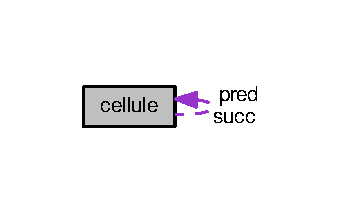
\includegraphics[width=164pt]{structcellule__coll__graph}
\end{center}
\end{figure}
\subsection*{Attributs publics}
\begin{DoxyCompactItemize}
\item 
\hypertarget{structcellule_a46ba624e4adf1dbb4dab081f8f2efdd0}{int {\bfseries val}}\label{structcellule_a46ba624e4adf1dbb4dab081f8f2efdd0}

\item 
\hypertarget{structcellule_a5dd827f4ec5d2e8cea82760188a60282}{struct \hyperlink{structcellule}{cellule} $\ast$ {\bfseries pred}}\label{structcellule_a5dd827f4ec5d2e8cea82760188a60282}

\item 
\hypertarget{structcellule_ae9e386b73942def78d49b1fb48475fb4}{struct \hyperlink{structcellule}{cellule} $\ast$ {\bfseries succ}}\label{structcellule_ae9e386b73942def78d49b1fb48475fb4}

\end{DoxyCompactItemize}


\subsection{Description détaillée}


Définition à la ligne 7 du fichier cellule.\+hpp.



La documentation de cette structure a été générée à partir du fichier suivant \+:\begin{DoxyCompactItemize}
\item 
cellule.\+hpp\end{DoxyCompactItemize}

\hypertarget{structDataNode}{\section{Référence de la structure Data\+Node}
\label{structDataNode}\index{Data\+Node@{Data\+Node}}
}
\subsection*{Attributs publics}
\begin{DoxyCompactItemize}
\item 
\hypertarget{structDataNode_a99899d182e970cc844a0c6ab7e297b01}{Q\+Vector3\+D {\bfseries \+\_\+lumiere\+\_\+diffuse}}\label{structDataNode_a99899d182e970cc844a0c6ab7e297b01}

\item 
\hypertarget{structDataNode_aef89a41e0f53bc4201537c9603dbfa49}{std\+::vector$<$ std\+::pair$<$ G\+Luint, \\*
Col\+Geom $>$ $>$ {\bfseries \+\_\+list\+\_\+vao\+\_\+mesh}}\label{structDataNode_aef89a41e0f53bc4201537c9603dbfa49}

\item 
\hypertarget{structDataNode_a621d28bc18ab708e985e1c8e268ef096}{Q\+Font\+::\+Style\+Hint {\bfseries \+\_\+style\+\_\+font}}\label{structDataNode_a621d28bc18ab708e985e1c8e268ef096}

\item 
\hypertarget{structDataNode_aac4897ced26e415bb827583b196daeb1}{Q\+Color {\bfseries \+\_\+color\+\_\+font}}\label{structDataNode_aac4897ced26e415bb827583b196daeb1}

\end{DoxyCompactItemize}


\subsection{Description détaillée}


Définition à la ligne 28 du fichier scene.\+hpp.



La documentation de cette structure a été générée à partir du fichier suivant \+:\begin{DoxyCompactItemize}
\item 
\hyperlink{scene_8hpp}{scene.\+hpp}\end{DoxyCompactItemize}

\hypertarget{classFile}{\section{Référence de la classe File}
\label{classFile}\index{File@{File}}
}


Graphe de collaboration de File\+:\nopagebreak
\begin{figure}[H]
\begin{center}
\leavevmode
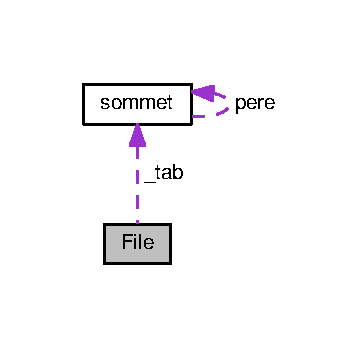
\includegraphics[width=172pt]{classFile__coll__graph}
\end{center}
\end{figure}
\subsection*{Fonctions membres publiques}
\begin{DoxyCompactItemize}
\item 
\hypertarget{classFile_a16cac2bfb7ce2d6d6fc85c8c6c1afb51}{{\bfseries File} (\hyperlink{classFile}{File} $\ast$)}\label{classFile_a16cac2bfb7ce2d6d6fc85c8c6c1afb51}

\item 
\hypertarget{classFile_a836c721d825c6d5593101fd3c2ef20fe}{int {\bfseries file\+\_\+vide} ()}\label{classFile_a836c721d825c6d5593101fd3c2ef20fe}

\item 
\hypertarget{classFile_a23378a28204e6df4fadf73cb91e99340}{void {\bfseries enfiler} (\hyperlink{structsommet}{sommet\+\_\+t} $\ast$)}\label{classFile_a23378a28204e6df4fadf73cb91e99340}

\item 
\hypertarget{classFile_a8c89b0bdf8a47894e784313eb15e5a46}{\hyperlink{structsommet}{sommet\+\_\+t} $\ast$ {\bfseries defiler} ()}\label{classFile_a8c89b0bdf8a47894e784313eb15e5a46}

\item 
\hypertarget{classFile_a1736d1e403772c3df0faabab421097c0}{void {\bfseries afficher\+\_\+file} ()}\label{classFile_a1736d1e403772c3df0faabab421097c0}

\end{DoxyCompactItemize}
\subsection*{Attributs publics}
\begin{DoxyCompactItemize}
\item 
\hypertarget{classFile_acfcf59c7a6cc50f3bb57ee66eef61476}{\hyperlink{structsommet}{sommet\+\_\+t} $\ast$$\ast$ {\bfseries \+\_\+tab}}\label{classFile_acfcf59c7a6cc50f3bb57ee66eef61476}

\item 
\hypertarget{classFile_ab47e6eafc5825a4cb0d7b95558c4cd1a}{int {\bfseries \+\_\+tete}}\label{classFile_ab47e6eafc5825a4cb0d7b95558c4cd1a}

\item 
\hypertarget{classFile_aaaf6f5329bd500cdc0db590d2594ab85}{int {\bfseries \+\_\+queue}}\label{classFile_aaaf6f5329bd500cdc0db590d2594ab85}

\end{DoxyCompactItemize}


\subsection{Description détaillée}


Définition à la ligne 14 du fichier file.\+hpp.



La documentation de cette classe a été générée à partir des fichiers suivants \+:\begin{DoxyCompactItemize}
\item 
file.\+hpp\item 
file.\+cpp\end{DoxyCompactItemize}

\hypertarget{classGraphe}{\section{Référence de la classe Graphe}
\label{classGraphe}\index{Graphe@{Graphe}}
}


Classe gerant la structure de donnée de graphe.  




{\ttfamily \#include $<$graphe.\+hpp$>$}



Graphe d'héritage de Graphe\+:\nopagebreak
\begin{figure}[H]
\begin{center}
\leavevmode
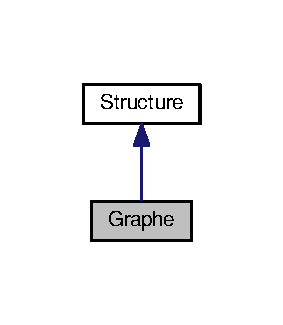
\includegraphics[width=136pt]{classGraphe__inherit__graph}
\end{center}
\end{figure}


Graphe de collaboration de Graphe\+:\nopagebreak
\begin{figure}[H]
\begin{center}
\leavevmode
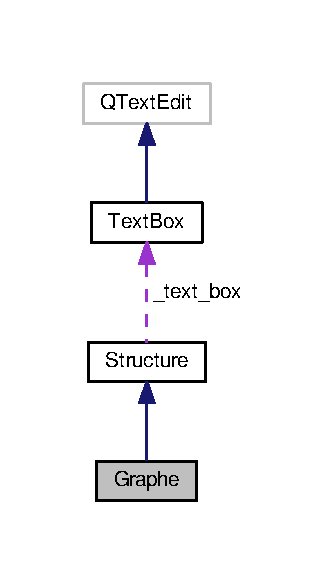
\includegraphics[width=136pt]{classGraphe__coll__graph}
\end{center}
\end{figure}
\subsection*{Fonctions membres publiques}
\begin{DoxyCompactItemize}
\item 
\hyperlink{classGraphe_a3d3949338bc93bf4edcfdc7310e4234f}{Graphe} (std\+::string path)
\begin{DoxyCompactList}\small\item\em Constructeur de la structure de graphe. \end{DoxyCompactList}\item 
\hypertarget{classGraphe_a673c897db564767e9ace7169a5357310}{\hyperlink{classGraphe_a673c897db564767e9ace7169a5357310}{$\sim$\+Graphe} ()}\label{classGraphe_a673c897db564767e9ace7169a5357310}

\begin{DoxyCompactList}\small\item\em Destructeur. \end{DoxyCompactList}\item 
void \hyperlink{classGraphe_a983bd623b721d7485805d252008d82f4}{charger} ()
\begin{DoxyCompactList}\small\item\em Chargement du graphe. \end{DoxyCompactList}\item 
\hypertarget{classGraphe_ae6dabb6a2315a88f7e0b35956d59a46b}{void \hyperlink{classGraphe_ae6dabb6a2315a88f7e0b35956d59a46b}{creer\+\_\+listes\+\_\+adjacences} ()}\label{classGraphe_ae6dabb6a2315a88f7e0b35956d59a46b}

\begin{DoxyCompactList}\small\item\em Creer liste d'adjacence. \end{DoxyCompactList}\item 
\hypertarget{classGraphe_ad6bf6139a94a026f4288e5ba1eb53e08}{void \hyperlink{classGraphe_ad6bf6139a94a026f4288e5ba1eb53e08}{creer\+\_\+matrice\+\_\+adjacences} ()}\label{classGraphe_ad6bf6139a94a026f4288e5ba1eb53e08}

\begin{DoxyCompactList}\small\item\em Creer matrice d'adjacence. \end{DoxyCompactList}\item 
\hypertarget{classGraphe_a01a623b6cfe3fcc38ef3ed0d3eb13226}{void \hyperlink{classGraphe_a01a623b6cfe3fcc38ef3ed0d3eb13226}{creer\+\_\+matrice\+\_\+laplace} ()}\label{classGraphe_a01a623b6cfe3fcc38ef3ed0d3eb13226}

\begin{DoxyCompactList}\small\item\em Creer matrice laplacienne. \end{DoxyCompactList}\item 
\hyperlink{structparcours__t}{parcours\+\_\+t} $\ast$ \hyperlink{classGraphe_ae824f4fe5eadd580272296b2e7cae561}{parcours\+\_\+largeur} (\hyperlink{structsommet}{sommet\+\_\+t} $\ast$s)
\begin{DoxyCompactList}\small\item\em Parcours en largeur. \end{DoxyCompactList}\item 
\hyperlink{structparcours__t}{parcours\+\_\+t} $\ast$ \hyperlink{classGraphe_a420e580d3803ee8ea7435ea7c15b2a91}{parcours\+\_\+profondeur} ()
\begin{DoxyCompactList}\small\item\em Parcours en profondeur. \end{DoxyCompactList}\item 
void \hyperlink{classGraphe_a8b6929c8f5869174c03f3ab2e4ec1fc8}{afficher\+\_\+parcours\+\_\+profondeur} ()
\begin{DoxyCompactList}\small\item\em Affichage du parcours en profondeur. \end{DoxyCompactList}\item 
void \hyperlink{classGraphe_a074adbc6a1f35fea18ede2a5be2ac767}{D\+F\+S\+\_\+visiter\+\_\+noeud} (\hyperlink{structsommet}{sommet\+\_\+t} $\ast$u, int $\ast$time, \hyperlink{structparcours__t}{parcours\+\_\+t} $\ast$p)
\begin{DoxyCompactList}\small\item\em Fonction interne à l'algorithme D\+F\+S. \end{DoxyCompactList}\item 
void \hyperlink{classGraphe_a0b150feac4a452b853ed6ed5be8d1c21}{afficher\+\_\+listes\+\_\+adjacences} (\hyperlink{structliste__adjacence__t}{liste\+\_\+adjacence\+\_\+t} $\ast$l)
\begin{DoxyCompactList}\small\item\em Affichage liste d'adjacences. \end{DoxyCompactList}\item 
void \hyperlink{classGraphe_a550984fee48fd6106686f45b09d7599d}{afficher\+\_\+matrice\+\_\+adjacences} (\hyperlink{structmatrice__adjacence__t}{matrice\+\_\+adjacence\+\_\+t} $\ast$l)
\begin{DoxyCompactList}\small\item\em Affichage matrice d'adjacences. \end{DoxyCompactList}\item 
void \hyperlink{classGraphe_a63126f39c2ab632b7a478bca7f902075}{afficher\+\_\+chemin} (\hyperlink{structsommet}{sommet\+\_\+t} $\ast$i, \hyperlink{structsommet}{sommet\+\_\+t} $\ast$j)
\begin{DoxyCompactList}\small\item\em Affichage chemin. \end{DoxyCompactList}\end{DoxyCompactItemize}
\subsection*{Membres hérités additionnels}


\subsection{Description détaillée}
Classe gerant la structure de donnée de graphe. 

Définition à la ligne 39 du fichier graphe.\+hpp.



\subsection{Documentation des constructeurs et destructeur}
\hypertarget{classGraphe_a3d3949338bc93bf4edcfdc7310e4234f}{\index{Graphe@{Graphe}!Graphe@{Graphe}}
\index{Graphe@{Graphe}!Graphe@{Graphe}}
\subsubsection[{Graphe}]{\setlength{\rightskip}{0pt plus 5cm}Graphe\+::\+Graphe (
\begin{DoxyParamCaption}
\item[{std\+::string}]{path}
\end{DoxyParamCaption}
)}}\label{classGraphe_a3d3949338bc93bf4edcfdc7310e4234f}


Constructeur de la structure de graphe. 

\hyperlink{classStructure}{Structure} de données permettant de manipuler des graphes et des algos de graphe. Le graphe ne sera pas charger, il est juste créer, pour le charger il faut appelé explicitement la fonction \hyperlink{classGraphe_a983bd623b721d7485805d252008d82f4}{charger()} 
\begin{DoxyParams}[1]{Paramètres}
\mbox{\tt in}  & {\em path} & chemin vers le fichier contenant le graphe \\
\hline
\end{DoxyParams}


Définition à la ligne 14 du fichier graphe.\+cpp.



\subsection{Documentation des fonctions membres}
\hypertarget{classGraphe_a63126f39c2ab632b7a478bca7f902075}{\index{Graphe@{Graphe}!afficher\+\_\+chemin@{afficher\+\_\+chemin}}
\index{afficher\+\_\+chemin@{afficher\+\_\+chemin}!Graphe@{Graphe}}
\subsubsection[{afficher\+\_\+chemin}]{\setlength{\rightskip}{0pt plus 5cm}void Graphe\+::afficher\+\_\+chemin (
\begin{DoxyParamCaption}
\item[{{\bf sommet\+\_\+t} $\ast$}]{i, }
\item[{{\bf sommet\+\_\+t} $\ast$}]{j}
\end{DoxyParamCaption}
)}}\label{classGraphe_a63126f39c2ab632b7a478bca7f902075}


Affichage chemin. 

affiche le chemin après un B\+F\+S, permet de voir le plus court chemin entre deux noeud passé en parametre 
\begin{DoxyParams}[1]{Paramètres}
\mbox{\tt in}  & {\em i} & sommet de depart \\
\hline
\mbox{\tt in}  & {\em j} & sommet d'arrivé \\
\hline
\end{DoxyParams}


Définition à la ligne 588 du fichier graphe.\+cpp.

\hypertarget{classGraphe_a0b150feac4a452b853ed6ed5be8d1c21}{\index{Graphe@{Graphe}!afficher\+\_\+listes\+\_\+adjacences@{afficher\+\_\+listes\+\_\+adjacences}}
\index{afficher\+\_\+listes\+\_\+adjacences@{afficher\+\_\+listes\+\_\+adjacences}!Graphe@{Graphe}}
\subsubsection[{afficher\+\_\+listes\+\_\+adjacences}]{\setlength{\rightskip}{0pt plus 5cm}void Graphe\+::afficher\+\_\+listes\+\_\+adjacences (
\begin{DoxyParamCaption}
\item[{{\bf liste\+\_\+adjacence\+\_\+t} $\ast$}]{l}
\end{DoxyParamCaption}
)}}\label{classGraphe_a0b150feac4a452b853ed6ed5be8d1c21}


Affichage liste d'adjacences. 

T\+O\+D\+O\+: utiliser operator$<$$<$ 

Définition à la ligne 426 du fichier graphe.\+cpp.

\hypertarget{classGraphe_a550984fee48fd6106686f45b09d7599d}{\index{Graphe@{Graphe}!afficher\+\_\+matrice\+\_\+adjacences@{afficher\+\_\+matrice\+\_\+adjacences}}
\index{afficher\+\_\+matrice\+\_\+adjacences@{afficher\+\_\+matrice\+\_\+adjacences}!Graphe@{Graphe}}
\subsubsection[{afficher\+\_\+matrice\+\_\+adjacences}]{\setlength{\rightskip}{0pt plus 5cm}void Graphe\+::afficher\+\_\+matrice\+\_\+adjacences (
\begin{DoxyParamCaption}
\item[{{\bf matrice\+\_\+adjacence\+\_\+t} $\ast$}]{l}
\end{DoxyParamCaption}
)}}\label{classGraphe_a550984fee48fd6106686f45b09d7599d}


Affichage matrice d'adjacences. 

T\+O\+D\+O\+: utiliser operator$<$$<$ 

Définition à la ligne 447 du fichier graphe.\+cpp.

\hypertarget{classGraphe_a8b6929c8f5869174c03f3ab2e4ec1fc8}{\index{Graphe@{Graphe}!afficher\+\_\+parcours\+\_\+profondeur@{afficher\+\_\+parcours\+\_\+profondeur}}
\index{afficher\+\_\+parcours\+\_\+profondeur@{afficher\+\_\+parcours\+\_\+profondeur}!Graphe@{Graphe}}
\subsubsection[{afficher\+\_\+parcours\+\_\+profondeur}]{\setlength{\rightskip}{0pt plus 5cm}void Graphe\+::afficher\+\_\+parcours\+\_\+profondeur (
\begin{DoxyParamCaption}
{}
\end{DoxyParamCaption}
)}}\label{classGraphe_a8b6929c8f5869174c03f3ab2e4ec1fc8}


Affichage du parcours en profondeur. 

Affiche le parcours en profondeur resultant, effectuer l'appel à cette fonction après avoir fait un parcours en profndeur 

Définition à la ligne 603 du fichier graphe.\+cpp.

\hypertarget{classGraphe_a983bd623b721d7485805d252008d82f4}{\index{Graphe@{Graphe}!charger@{charger}}
\index{charger@{charger}!Graphe@{Graphe}}
\subsubsection[{charger}]{\setlength{\rightskip}{0pt plus 5cm}void Graphe\+::charger (
\begin{DoxyParamCaption}
{}
\end{DoxyParamCaption}
)\hspace{0.3cm}{\ttfamily [virtual]}}}\label{classGraphe_a983bd623b721d7485805d252008d82f4}


Chargement du graphe. 

Chargement du graphe de maniere explicite à partir de l'appel de cette fonction 

Implémente \hyperlink{classStructure_ae99db977c0b38122644cf458ea3d5974}{Structure}.



Définition à la ligne 38 du fichier graphe.\+cpp.

\hypertarget{classGraphe_a074adbc6a1f35fea18ede2a5be2ac767}{\index{Graphe@{Graphe}!D\+F\+S\+\_\+visiter\+\_\+noeud@{D\+F\+S\+\_\+visiter\+\_\+noeud}}
\index{D\+F\+S\+\_\+visiter\+\_\+noeud@{D\+F\+S\+\_\+visiter\+\_\+noeud}!Graphe@{Graphe}}
\subsubsection[{D\+F\+S\+\_\+visiter\+\_\+noeud}]{\setlength{\rightskip}{0pt plus 5cm}void Graphe\+::\+D\+F\+S\+\_\+visiter\+\_\+noeud (
\begin{DoxyParamCaption}
\item[{{\bf sommet\+\_\+t} $\ast$}]{u, }
\item[{int $\ast$}]{time, }
\item[{{\bf parcours\+\_\+t} $\ast$}]{p}
\end{DoxyParamCaption}
)}}\label{classGraphe_a074adbc6a1f35fea18ede2a5be2ac767}


Fonction interne à l'algorithme D\+F\+S. 


\begin{DoxyParams}[1]{Paramètres}
\mbox{\tt in}  & {\em u} & sommet à visiter \\
\hline
\mbox{\tt in}  & {\em time} & date à laquelle on visite le noeud \\
\hline
\mbox{\tt in}  & {\em p} & parcours dans lequel est integré la visite du noeud \\
\hline
\end{DoxyParams}


Définition à la ligne 639 du fichier graphe.\+cpp.

\hypertarget{classGraphe_ae824f4fe5eadd580272296b2e7cae561}{\index{Graphe@{Graphe}!parcours\+\_\+largeur@{parcours\+\_\+largeur}}
\index{parcours\+\_\+largeur@{parcours\+\_\+largeur}!Graphe@{Graphe}}
\subsubsection[{parcours\+\_\+largeur}]{\setlength{\rightskip}{0pt plus 5cm}{\bf parcours\+\_\+t} $\ast$ Graphe\+::parcours\+\_\+largeur (
\begin{DoxyParamCaption}
\item[{{\bf sommet\+\_\+t} $\ast$}]{s}
\end{DoxyParamCaption}
)}}\label{classGraphe_ae824f4fe5eadd580272296b2e7cae561}


Parcours en largeur. 

Algorithme B\+F\+S, parcours en largeur sur le graphe courant 
\begin{DoxyParams}[1]{Paramètres}
\mbox{\tt in}  & {\em s} & sommet de depart pour le parcours en largeur \\
\hline
\mbox{\tt out}  & {\em parcours} & en largeur resultant \\
\hline
\end{DoxyParams}


Définition à la ligne 523 du fichier graphe.\+cpp.

\hypertarget{classGraphe_a420e580d3803ee8ea7435ea7c15b2a91}{\index{Graphe@{Graphe}!parcours\+\_\+profondeur@{parcours\+\_\+profondeur}}
\index{parcours\+\_\+profondeur@{parcours\+\_\+profondeur}!Graphe@{Graphe}}
\subsubsection[{parcours\+\_\+profondeur}]{\setlength{\rightskip}{0pt plus 5cm}{\bf parcours\+\_\+t} $\ast$ Graphe\+::parcours\+\_\+profondeur (
\begin{DoxyParamCaption}
{}
\end{DoxyParamCaption}
)}}\label{classGraphe_a420e580d3803ee8ea7435ea7c15b2a91}


Parcours en profondeur. 

Algorithme D\+F\+S, parcours en profondeur sur le graphe courant 
\begin{DoxyParams}[1]{Paramètres}
\mbox{\tt out}  & {\em parcours} & en largeur resultant \\
\hline
\end{DoxyParams}


Définition à la ligne 612 du fichier graphe.\+cpp.



La documentation de cette classe a été générée à partir des fichiers suivants \+:\begin{DoxyCompactItemize}
\item 
\hyperlink{graphe_8hpp}{graphe.\+hpp}\item 
\hyperlink{graphe_8cpp}{graphe.\+cpp}\end{DoxyCompactItemize}

\hypertarget{classListe}{\section{Référence de la classe Liste}
\label{classListe}\index{Liste@{Liste}}
}


Graphe de collaboration de Liste\+:\nopagebreak
\begin{figure}[H]
\begin{center}
\leavevmode
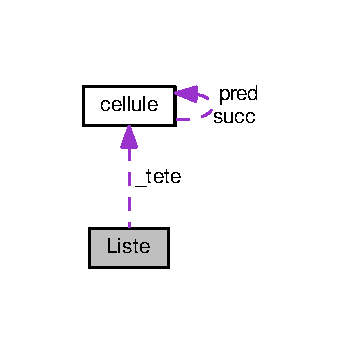
\includegraphics[width=164pt]{classListe__coll__graph}
\end{center}
\end{figure}
\subsection*{Fonctions membres publiques}
\begin{DoxyCompactItemize}
\item 
\hypertarget{classListe_a0b5ce6f952058cf3d9b124c76c508b37}{void {\bfseries inserer} (\hyperlink{structcellule}{cellule\+\_\+t} $\ast$)}\label{classListe_a0b5ce6f952058cf3d9b124c76c508b37}

\item 
\hypertarget{classListe_a37e9a70e70ffbdf709494f5eda93b2c1}{\hyperlink{structcellule}{cellule\+\_\+t} $\ast$ {\bfseries rechercher} (int)}\label{classListe_a37e9a70e70ffbdf709494f5eda93b2c1}

\item 
\hypertarget{classListe_ad49550c8526fdc22cfb99da6e7741978}{void {\bfseries supprimer} (\hyperlink{structcellule}{cellule\+\_\+t} $\ast$)}\label{classListe_ad49550c8526fdc22cfb99da6e7741978}

\item 
\hypertarget{classListe_aadf373e279e6786bca499f5f8953548f}{int {\bfseries compter\+\_\+liste} ()}\label{classListe_aadf373e279e6786bca499f5f8953548f}

\item 
\hypertarget{classListe_adcec4235c891e6dfea8f96f3d405c048}{void {\bfseries afficher\+\_\+liste} ()}\label{classListe_adcec4235c891e6dfea8f96f3d405c048}

\end{DoxyCompactItemize}
\subsection*{Attributs publics}
\begin{DoxyCompactItemize}
\item 
\hypertarget{classListe_a203aaf18ff964be5f4bf927a7257e146}{\hyperlink{structcellule}{cellule\+\_\+t} $\ast$ {\bfseries \+\_\+tete}}\label{classListe_a203aaf18ff964be5f4bf927a7257e146}

\end{DoxyCompactItemize}


\subsection{Description détaillée}


Définition à la ligne 7 du fichier liste.\+hpp.



La documentation de cette classe a été générée à partir des fichiers suivants \+:\begin{DoxyCompactItemize}
\item 
liste.\+hpp\item 
liste.\+cpp\end{DoxyCompactItemize}

\hypertarget{structliste__adjacence__t}{\section{Référence de la structure liste\+\_\+adjacence\+\_\+t}
\label{structliste__adjacence__t}\index{liste\+\_\+adjacence\+\_\+t@{liste\+\_\+adjacence\+\_\+t}}
}


Graphe de collaboration de liste\+\_\+adjacence\+\_\+t\+:\nopagebreak
\begin{figure}[H]
\begin{center}
\leavevmode
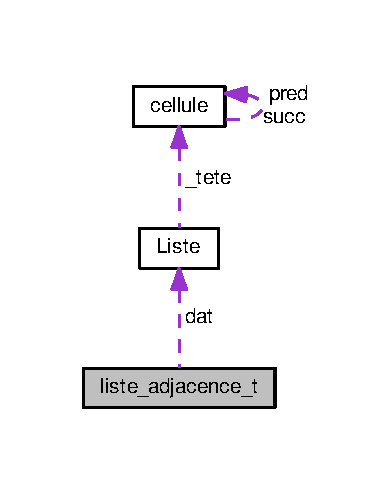
\includegraphics[width=188pt]{structliste__adjacence__t__coll__graph}
\end{center}
\end{figure}
\subsection*{Attributs publics}
\begin{DoxyCompactItemize}
\item 
\hypertarget{structliste__adjacence__t_aa2ce2755fe745acafa83b31ef058e2bf}{\hyperlink{classListe}{Liste} $\ast$$\ast$ {\bfseries dat}}\label{structliste__adjacence__t_aa2ce2755fe745acafa83b31ef058e2bf}

\item 
\hypertarget{structliste__adjacence__t_a9eb23de3f625a350ee1eec6f7384c8ab}{int {\bfseries nbr\+A}}\label{structliste__adjacence__t_a9eb23de3f625a350ee1eec6f7384c8ab}

\item 
\hypertarget{structliste__adjacence__t_a2b1c14efef06ec98f7c600dc74bb85ca}{int {\bfseries nbr\+S}}\label{structliste__adjacence__t_a2b1c14efef06ec98f7c600dc74bb85ca}

\end{DoxyCompactItemize}


\subsection{Description détaillée}


Définition à la ligne 13 du fichier graphe.\+hpp.



La documentation de cette structure a été générée à partir du fichier suivant \+:\begin{DoxyCompactItemize}
\item 
\hyperlink{graphe_8hpp}{graphe.\+hpp}\end{DoxyCompactItemize}

\hypertarget{classMainWindow}{\section{Référence de la classe Main\+Window}
\label{classMainWindow}\index{Main\+Window@{Main\+Window}}
}


classe gerant le placement et interactions des principaux widgets dans la fenetre principale  




{\ttfamily \#include $<$mainwindow.\+hpp$>$}



Graphe d'héritage de Main\+Window\+:\nopagebreak
\begin{figure}[H]
\begin{center}
\leavevmode
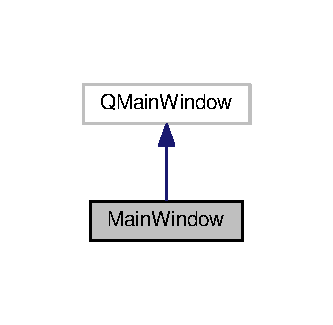
\includegraphics[width=160pt]{classMainWindow__inherit__graph}
\end{center}
\end{figure}


Graphe de collaboration de Main\+Window\+:\nopagebreak
\begin{figure}[H]
\begin{center}
\leavevmode
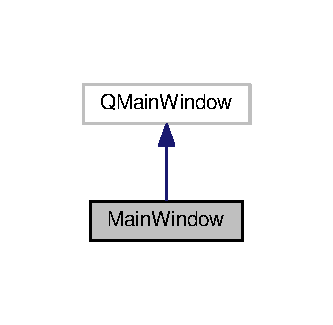
\includegraphics[width=160pt]{classMainWindow__coll__graph}
\end{center}
\end{figure}
\subsection*{Fonctions membres publiques}
\begin{DoxyCompactItemize}
\item 
\hyperlink{classMainWindow_a8b244be8b7b7db1b08de2a2acb9409db}{Main\+Window} (Q\+Widget $\ast$parent=0)
\begin{DoxyCompactList}\small\item\em Constructeur de la fenetre principale. \end{DoxyCompactList}\item 
void \hyperlink{classMainWindow_a255a5c38fd871c168fac835692871d62}{selection\+\_\+graphe} ()
\begin{DoxyCompactList}\small\item\em Selection d'un graphe. \end{DoxyCompactList}\item 
void \hyperlink{classMainWindow_a00c50c04982c1f685f281606e8e1fff5}{charger\+\_\+menu} ()
\begin{DoxyCompactList}\small\item\em Chargeur du menu. \end{DoxyCompactList}\item 
void \hyperlink{classMainWindow_a6d34935ca23b2c54a784ae2b7944a1ad}{charger\+\_\+opengl} ()
\begin{DoxyCompactList}\small\item\em Chargeur Open\+G\+L. \end{DoxyCompactList}\end{DoxyCompactItemize}


\subsection{Description détaillée}
classe gerant le placement et interactions des principaux widgets dans la fenetre principale 

Définition à la ligne 38 du fichier mainwindow.\+hpp.



\subsection{Documentation des constructeurs et destructeur}
\hypertarget{classMainWindow_a8b244be8b7b7db1b08de2a2acb9409db}{\index{Main\+Window@{Main\+Window}!Main\+Window@{Main\+Window}}
\index{Main\+Window@{Main\+Window}!Main\+Window@{Main\+Window}}
\subsubsection[{Main\+Window}]{\setlength{\rightskip}{0pt plus 5cm}Main\+Window\+::\+Main\+Window (
\begin{DoxyParamCaption}
\item[{Q\+Widget $\ast$}]{parent = {\ttfamily 0}}
\end{DoxyParamCaption}
)}}\label{classMainWindow_a8b244be8b7b7db1b08de2a2acb9409db}


Constructeur de la fenetre principale. 

il s'agit de la fenetre principale, elle n'a pas de parent, mais on laisse le parametre par commodité 
\begin{DoxyParams}[1]{Paramètres}
\mbox{\tt in}  & {\em parent} & le widget parent \\
\hline
\end{DoxyParams}


Définition à la ligne 7 du fichier mainwindow.\+cpp.



\subsection{Documentation des fonctions membres}
\hypertarget{classMainWindow_a00c50c04982c1f685f281606e8e1fff5}{\index{Main\+Window@{Main\+Window}!charger\+\_\+menu@{charger\+\_\+menu}}
\index{charger\+\_\+menu@{charger\+\_\+menu}!Main\+Window@{Main\+Window}}
\subsubsection[{charger\+\_\+menu}]{\setlength{\rightskip}{0pt plus 5cm}void Main\+Window\+::charger\+\_\+menu (
\begin{DoxyParamCaption}
{}
\end{DoxyParamCaption}
)\hspace{0.3cm}{\ttfamily [inline]}}}\label{classMainWindow_a00c50c04982c1f685f281606e8e1fff5}


Chargeur du menu. 

Appelé lors de la construction de la fenetre principale, construit la barre de menu, et associe les signaux aux actions 

Définition à la ligne 66 du fichier mainwindow.\+cpp.

\hypertarget{classMainWindow_a6d34935ca23b2c54a784ae2b7944a1ad}{\index{Main\+Window@{Main\+Window}!charger\+\_\+opengl@{charger\+\_\+opengl}}
\index{charger\+\_\+opengl@{charger\+\_\+opengl}!Main\+Window@{Main\+Window}}
\subsubsection[{charger\+\_\+opengl}]{\setlength{\rightskip}{0pt plus 5cm}void Main\+Window\+::charger\+\_\+opengl (
\begin{DoxyParamCaption}
{}
\end{DoxyParamCaption}
)\hspace{0.3cm}{\ttfamily [inline]}}}\label{classMainWindow_a6d34935ca23b2c54a784ae2b7944a1ad}


Chargeur Open\+G\+L. 

Appelé lors de la construction de la fenetre principale, cette fonction appelle le constructeur de \hyperlink{classSceneGL}{Scene\+G\+L} créant le widget Open\+G\+L qui sera integré dans la fenetre principale 

Définition à la ligne 116 du fichier mainwindow.\+cpp.

\hypertarget{classMainWindow_a255a5c38fd871c168fac835692871d62}{\index{Main\+Window@{Main\+Window}!selection\+\_\+graphe@{selection\+\_\+graphe}}
\index{selection\+\_\+graphe@{selection\+\_\+graphe}!Main\+Window@{Main\+Window}}
\subsubsection[{selection\+\_\+graphe}]{\setlength{\rightskip}{0pt plus 5cm}void Main\+Window\+::selection\+\_\+graphe (
\begin{DoxyParamCaption}
{}
\end{DoxyParamCaption}
)}}\label{classMainWindow_a255a5c38fd871c168fac835692871d62}


Selection d'un graphe. 

Appelé lors de la reception d'un signal emis par l'utilisateur lorsqu'il demande d'ouvrir un nouveau graphe dans le menu. Cette fonction ouvre une boite de dialogue permettant de selectionner le graphe, puis va créer une structure de graphe à partir du fichier sélectionné. 

Définition à la ligne 34 du fichier mainwindow.\+cpp.



La documentation de cette classe a été générée à partir des fichiers suivants \+:\begin{DoxyCompactItemize}
\item 
\hyperlink{mainwindow_8hpp}{mainwindow.\+hpp}\item 
\hyperlink{mainwindow_8cpp}{mainwindow.\+cpp}\end{DoxyCompactItemize}

\hypertarget{structmatrice__adjacence__t}{\section{Référence de la structure matrice\+\_\+adjacence\+\_\+t}
\label{structmatrice__adjacence__t}\index{matrice\+\_\+adjacence\+\_\+t@{matrice\+\_\+adjacence\+\_\+t}}
}
\subsection*{Attributs publics}
\begin{DoxyCompactItemize}
\item 
\hypertarget{structmatrice__adjacence__t_a22789ec00178354cf7d10af8afa4bd10}{int $\ast$$\ast$ {\bfseries dat}}\label{structmatrice__adjacence__t_a22789ec00178354cf7d10af8afa4bd10}

\item 
\hypertarget{structmatrice__adjacence__t_a27d3582be114699610adb4c332ce5448}{int {\bfseries nbr\+A}}\label{structmatrice__adjacence__t_a27d3582be114699610adb4c332ce5448}

\item 
\hypertarget{structmatrice__adjacence__t_a9d7874868df1751f3f65a5a852d7e0a5}{int {\bfseries nbr\+S}}\label{structmatrice__adjacence__t_a9d7874868df1751f3f65a5a852d7e0a5}

\end{DoxyCompactItemize}


\subsection{Description détaillée}


Définition à la ligne 27 du fichier graphe.\+hpp.



La documentation de cette structure a été générée à partir du fichier suivant \+:\begin{DoxyCompactItemize}
\item 
\hyperlink{graphe_8hpp}{graphe.\+hpp}\end{DoxyCompactItemize}

\hypertarget{structmatrice__laplace__t}{\section{Référence de la structure matrice\+\_\+laplace\+\_\+t}
\label{structmatrice__laplace__t}\index{matrice\+\_\+laplace\+\_\+t@{matrice\+\_\+laplace\+\_\+t}}
}
\subsection*{Attributs publics}
\begin{DoxyCompactItemize}
\item 
\hypertarget{structmatrice__laplace__t_a3f58ff72f8d8e5b8f154e369916d7d08}{int $\ast$$\ast$ {\bfseries dat}}\label{structmatrice__laplace__t_a3f58ff72f8d8e5b8f154e369916d7d08}

\item 
\hypertarget{structmatrice__laplace__t_aa88d77ffa32b29613bf571afe3ea03e0}{int {\bfseries nbr\+A}}\label{structmatrice__laplace__t_aa88d77ffa32b29613bf571afe3ea03e0}

\item 
\hypertarget{structmatrice__laplace__t_a93d1312a981c2f318811735736d3d85c}{int {\bfseries nbr\+S}}\label{structmatrice__laplace__t_a93d1312a981c2f318811735736d3d85c}

\end{DoxyCompactItemize}


\subsection{Description détaillée}


Définition à la ligne 19 du fichier graphe.\+hpp.



La documentation de cette structure a été générée à partir du fichier suivant \+:\begin{DoxyCompactItemize}
\item 
\hyperlink{graphe_8hpp}{graphe.\+hpp}\end{DoxyCompactItemize}

\hypertarget{structparam__lux}{\section{Référence de la structure param\+\_\+lux}
\label{structparam__lux}\index{param\+\_\+lux@{param\+\_\+lux}}
}
\subsection*{Attributs publics}
\begin{DoxyCompactItemize}
\item 
\hypertarget{structparam__lux_a18a60a5f3b290f21a1f9b81dbdc0275c}{glm\+::vec4 {\bfseries diffuse\+\_\+intensity}}\label{structparam__lux_a18a60a5f3b290f21a1f9b81dbdc0275c}

\item 
\hypertarget{structparam__lux_ab716533c7c60d7fe5b610ac81ac4855d}{glm\+::vec4 {\bfseries ambient\+\_\+intensity}}\label{structparam__lux_ab716533c7c60d7fe5b610ac81ac4855d}

\item 
\hypertarget{structparam__lux_a29d5fb59ee1d0b47c44777f23ff10809}{glm\+::vec4 {\bfseries light\+\_\+direction}}\label{structparam__lux_a29d5fb59ee1d0b47c44777f23ff10809}

\end{DoxyCompactItemize}


\subsection{Description détaillée}


Définition à la ligne 25 du fichier scene.\+cpp.



La documentation de cette structure a été générée à partir du fichier suivant \+:\begin{DoxyCompactItemize}
\item 
\hyperlink{scene_8cpp}{scene.\+cpp}\end{DoxyCompactItemize}

\hypertarget{structparcours__t}{\section{Référence de la structure parcours\+\_\+t}
\label{structparcours__t}\index{parcours\+\_\+t@{parcours\+\_\+t}}
}


Graphe de collaboration de parcours\+\_\+t\+:\nopagebreak
\begin{figure}[H]
\begin{center}
\leavevmode
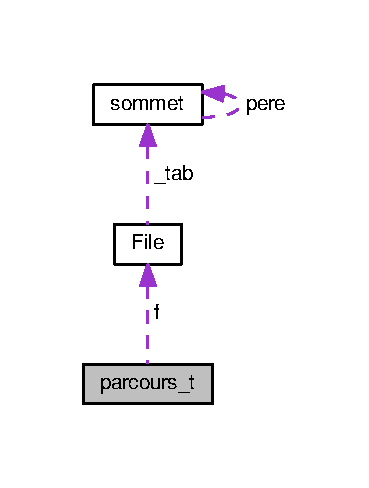
\includegraphics[width=177pt]{structparcours__t__coll__graph}
\end{center}
\end{figure}
\subsection*{Attributs publics}
\begin{DoxyCompactItemize}
\item 
\hypertarget{structparcours__t_a0bb6da520f00c8404b61c1e5c7cf577b}{\hyperlink{classFile}{File} $\ast$ {\bfseries f}}\label{structparcours__t_a0bb6da520f00c8404b61c1e5c7cf577b}

\end{DoxyCompactItemize}


\subsection{Description détaillée}


Définition à la ligne 33 du fichier graphe.\+hpp.



La documentation de cette structure a été générée à partir du fichier suivant \+:\begin{DoxyCompactItemize}
\item 
\hyperlink{graphe_8hpp}{graphe.\+hpp}\end{DoxyCompactItemize}

\hypertarget{classSceneGL}{\section{Référence de la classe Scene\+G\+L}
\label{classSceneGL}\index{Scene\+G\+L@{Scene\+G\+L}}
}


classe gerant le contexte Open\+G\+L de l'application  




{\ttfamily \#include $<$scene.\+hpp$>$}



Graphe d'héritage de Scene\+G\+L\+:\nopagebreak
\begin{figure}[H]
\begin{center}
\leavevmode
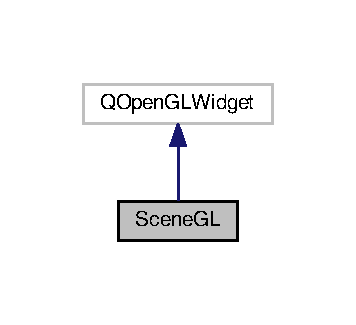
\includegraphics[width=171pt]{classSceneGL__inherit__graph}
\end{center}
\end{figure}


Graphe de collaboration de Scene\+G\+L\+:\nopagebreak
\begin{figure}[H]
\begin{center}
\leavevmode
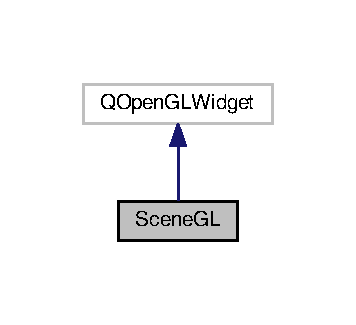
\includegraphics[width=171pt]{classSceneGL__coll__graph}
\end{center}
\end{figure}
\subsection*{Fonctions membres publiques}
\begin{DoxyCompactItemize}
\item 
\hyperlink{classSceneGL_a5bc9486686f1a7cbcbca2ecf7a55ad09}{Scene\+G\+L} (std\+::string vertex\+\_\+shad, std\+::string fragment\+\_\+shad, Q\+Widget $\ast$parent=0, \hyperlink{classStructure}{Structure} $\ast$str=nullptr, Qt\+::\+Window\+Flags f=0)
\begin{DoxyCompactList}\small\item\em Constructeur de la scene G\+L. \end{DoxyCompactList}\item 
\hyperlink{classSceneGL_a0e4266dea6edaca8b5274b9d74e4fe56}{$\sim$\+Scene\+G\+L} ()
\begin{DoxyCompactList}\small\item\em Destructeur. \end{DoxyCompactList}\item 
void \hyperlink{classSceneGL_ad81e01d02213ca0bdbec735260408f23}{initialize\+G\+L} ()
\begin{DoxyCompactList}\small\item\em Initialise le contexte Open\+G\+L. \end{DoxyCompactList}\item 
void \hyperlink{classSceneGL_a70997c4a649f1b17710a14549bf6990b}{cleanup\+G\+L} ()
\begin{DoxyCompactList}\small\item\em Fonction de formattage. \end{DoxyCompactList}\item 
void \hyperlink{classSceneGL_a45a49b85da1c7cb756b622c97028bf1b}{resize\+G\+L} (int w, int h)
\begin{DoxyCompactList}\small\item\em Fonction de redimensionnement. \end{DoxyCompactList}\item 
void \hyperlink{classSceneGL_a4e3548c5440b13ff4fe0fb76bc766276}{paint\+G\+L} ()
\begin{DoxyCompactList}\small\item\em Fonction qui est appelé quand le widget a besoin d'etre repaint. \end{DoxyCompactList}\item 
void \hyperlink{classSceneGL_a8ee0b8b7fdabc17840b1c037759b4dc6}{Zoompos} ()
\begin{DoxyCompactList}\small\item\em Fonction de zoom avant de la camera. \end{DoxyCompactList}\item 
void \hyperlink{classSceneGL_ad003ab949696de713f2f0abaed4c7558}{Zoomneg} ()
\begin{DoxyCompactList}\small\item\em Fonction de zoom arriere de la camera. \end{DoxyCompactList}\item 
\hyperlink{classStructure}{Structure} $\ast$ \hyperlink{classSceneGL_a53d49272e92f87c42ee726604430e778}{get\+\_\+structure} ()
\begin{DoxyCompactList}\small\item\em Getters de la structure. \end{DoxyCompactList}\item 
void \hyperlink{classSceneGL_a409672c6feccc6d1d6bc5dcdcfa7e9c6}{charger\+\_\+contenu\+\_\+graphique} ()
\begin{DoxyCompactList}\small\item\em Charger contenu graphique. \end{DoxyCompactList}\end{DoxyCompactItemize}


\subsection{Description détaillée}
classe gerant le contexte Open\+G\+L de l'application 

Définition à la ligne 27 du fichier scene.\+hpp.



\subsection{Documentation des constructeurs et destructeur}
\hypertarget{classSceneGL_a5bc9486686f1a7cbcbca2ecf7a55ad09}{\index{Scene\+G\+L@{Scene\+G\+L}!Scene\+G\+L@{Scene\+G\+L}}
\index{Scene\+G\+L@{Scene\+G\+L}!Scene\+G\+L@{Scene\+G\+L}}
\subsubsection[{Scene\+G\+L}]{\setlength{\rightskip}{0pt plus 5cm}Scene\+G\+L\+::\+Scene\+G\+L (
\begin{DoxyParamCaption}
\item[{std\+::string}]{vertex\+\_\+shad, }
\item[{std\+::string}]{fragment\+\_\+shad, }
\item[{Q\+Widget $\ast$}]{parent = {\ttfamily 0}, }
\item[{{\bf Structure} $\ast$}]{str = {\ttfamily nullptr}, }
\item[{Qt\+::\+Window\+Flags}]{f = {\ttfamily 0}}
\end{DoxyParamCaption}
)}}\label{classSceneGL_a5bc9486686f1a7cbcbca2ecf7a55ad09}


Constructeur de la scene G\+L. 

il s'agit de la fenetre principale, elle n'a pas de parent, mais on laisse le parametre par commodité 
\begin{DoxyParams}[1]{Paramètres}
\mbox{\tt in}  & {\em vertex\+\_\+shad} & le vertex shaders \\
\hline
\mbox{\tt in}  & {\em fragment\+\_\+shad} & le fragment shaders \\
\hline
\mbox{\tt in}  & {\em parent} & le widget parent où sera contenu le contexte Open\+G\+L \\
\hline
\mbox{\tt in}  & {\em str} & la structure \\
\hline
\mbox{\tt in}  & {\em flags} & flags de widget \\
\hline
\end{DoxyParams}


Définition à la ligne 20 du fichier scene.\+cpp.

\hypertarget{classSceneGL_a0e4266dea6edaca8b5274b9d74e4fe56}{\index{Scene\+G\+L@{Scene\+G\+L}!````~Scene\+G\+L@{$\sim$\+Scene\+G\+L}}
\index{````~Scene\+G\+L@{$\sim$\+Scene\+G\+L}!Scene\+G\+L@{Scene\+G\+L}}
\subsubsection[{$\sim$\+Scene\+G\+L}]{\setlength{\rightskip}{0pt plus 5cm}Scene\+G\+L\+::$\sim$\+Scene\+G\+L (
\begin{DoxyParamCaption}
{}
\end{DoxyParamCaption}
)}}\label{classSceneGL_a0e4266dea6edaca8b5274b9d74e4fe56}


Destructeur. 

Destructeur 

Définition à la ligne 284 du fichier scene.\+cpp.



\subsection{Documentation des fonctions membres}
\hypertarget{classSceneGL_a409672c6feccc6d1d6bc5dcdcfa7e9c6}{\index{Scene\+G\+L@{Scene\+G\+L}!charger\+\_\+contenu\+\_\+graphique@{charger\+\_\+contenu\+\_\+graphique}}
\index{charger\+\_\+contenu\+\_\+graphique@{charger\+\_\+contenu\+\_\+graphique}!Scene\+G\+L@{Scene\+G\+L}}
\subsubsection[{charger\+\_\+contenu\+\_\+graphique}]{\setlength{\rightskip}{0pt plus 5cm}void Scene\+G\+L\+::charger\+\_\+contenu\+\_\+graphique (
\begin{DoxyParamCaption}
{}
\end{DoxyParamCaption}
)}}\label{classSceneGL_a409672c6feccc6d1d6bc5dcdcfa7e9c6}


Charger contenu graphique. 

Charge le contenu graphique à afficher dans le contexte Open\+G\+L 

Définition à la ligne 128 du fichier scene.\+cpp.

\hypertarget{classSceneGL_a70997c4a649f1b17710a14549bf6990b}{\index{Scene\+G\+L@{Scene\+G\+L}!cleanup\+G\+L@{cleanup\+G\+L}}
\index{cleanup\+G\+L@{cleanup\+G\+L}!Scene\+G\+L@{Scene\+G\+L}}
\subsubsection[{cleanup\+G\+L}]{\setlength{\rightskip}{0pt plus 5cm}void Scene\+G\+L\+::cleanup\+G\+L (
\begin{DoxyParamCaption}
{}
\end{DoxyParamCaption}
)}}\label{classSceneGL_a70997c4a649f1b17710a14549bf6990b}


Fonction de formattage. 

Cette fonction supprime les identifiants de shaders et vide les buffers 

Définition à la ligne 194 du fichier scene.\+cpp.

\hypertarget{classSceneGL_a53d49272e92f87c42ee726604430e778}{\index{Scene\+G\+L@{Scene\+G\+L}!get\+\_\+structure@{get\+\_\+structure}}
\index{get\+\_\+structure@{get\+\_\+structure}!Scene\+G\+L@{Scene\+G\+L}}
\subsubsection[{get\+\_\+structure}]{\setlength{\rightskip}{0pt plus 5cm}{\bf Structure} $\ast$ Scene\+G\+L\+::get\+\_\+structure (
\begin{DoxyParamCaption}
{}
\end{DoxyParamCaption}
)}}\label{classSceneGL_a53d49272e92f87c42ee726604430e778}


Getters de la structure. 

Getters de la structure chargé dans la scene Open\+G\+L courante 

Définition à la ligne 267 du fichier scene.\+cpp.

\hypertarget{classSceneGL_ad81e01d02213ca0bdbec735260408f23}{\index{Scene\+G\+L@{Scene\+G\+L}!initialize\+G\+L@{initialize\+G\+L}}
\index{initialize\+G\+L@{initialize\+G\+L}!Scene\+G\+L@{Scene\+G\+L}}
\subsubsection[{initialize\+G\+L}]{\setlength{\rightskip}{0pt plus 5cm}void Scene\+G\+L\+::initialize\+G\+L (
\begin{DoxyParamCaption}
{}
\end{DoxyParamCaption}
)}}\label{classSceneGL_ad81e01d02213ca0bdbec735260408f23}


Initialise le contexte Open\+G\+L. 

Cette fonction est appelé une fois avant le premier appel à paint\+G\+L ou à resize\+G\+L 

Définition à la ligne 52 du fichier scene.\+cpp.

\hypertarget{classSceneGL_a4e3548c5440b13ff4fe0fb76bc766276}{\index{Scene\+G\+L@{Scene\+G\+L}!paint\+G\+L@{paint\+G\+L}}
\index{paint\+G\+L@{paint\+G\+L}!Scene\+G\+L@{Scene\+G\+L}}
\subsubsection[{paint\+G\+L}]{\setlength{\rightskip}{0pt plus 5cm}void Scene\+G\+L\+::paint\+G\+L (
\begin{DoxyParamCaption}
{}
\end{DoxyParamCaption}
)}}\label{classSceneGL_a4e3548c5440b13ff4fe0fb76bc766276}


Fonction qui est appelé quand le widget a besoin d'etre repaint. 

Cette fonction est appelé une fois avant le premier appel à paint\+G\+L ou à resize\+G\+L 

Définition à la ligne 224 du fichier scene.\+cpp.

\hypertarget{classSceneGL_a45a49b85da1c7cb756b622c97028bf1b}{\index{Scene\+G\+L@{Scene\+G\+L}!resize\+G\+L@{resize\+G\+L}}
\index{resize\+G\+L@{resize\+G\+L}!Scene\+G\+L@{Scene\+G\+L}}
\subsubsection[{resize\+G\+L}]{\setlength{\rightskip}{0pt plus 5cm}void Scene\+G\+L\+::resize\+G\+L (
\begin{DoxyParamCaption}
\item[{int}]{w, }
\item[{int}]{h}
\end{DoxyParamCaption}
)}}\label{classSceneGL_a45a49b85da1c7cb756b622c97028bf1b}


Fonction de redimensionnement. 

Cette fonction est appelé lorsque le widget conteneur du contexte Open\+G\+L est redimensionné 
\begin{DoxyParams}[1]{Paramètres}
\mbox{\tt in}  & {\em w} & nouvelle dimension de largeur \\
\hline
\mbox{\tt in}  & {\em h} & nouvelle dimension de hauteur \\
\hline
\end{DoxyParams}


Définition à la ligne 219 du fichier scene.\+cpp.

\hypertarget{classSceneGL_ad003ab949696de713f2f0abaed4c7558}{\index{Scene\+G\+L@{Scene\+G\+L}!Zoomneg@{Zoomneg}}
\index{Zoomneg@{Zoomneg}!Scene\+G\+L@{Scene\+G\+L}}
\subsubsection[{Zoomneg}]{\setlength{\rightskip}{0pt plus 5cm}void Scene\+G\+L\+::\+Zoomneg (
\begin{DoxyParamCaption}
{}
\end{DoxyParamCaption}
)}}\label{classSceneGL_ad003ab949696de713f2f0abaed4c7558}


Fonction de zoom arriere de la camera. 

Fonction appelé lors d'un zoom arriere commandé par l'I\+H\+M 

Définition à la ligne 278 du fichier scene.\+cpp.

\hypertarget{classSceneGL_a8ee0b8b7fdabc17840b1c037759b4dc6}{\index{Scene\+G\+L@{Scene\+G\+L}!Zoompos@{Zoompos}}
\index{Zoompos@{Zoompos}!Scene\+G\+L@{Scene\+G\+L}}
\subsubsection[{Zoompos}]{\setlength{\rightskip}{0pt plus 5cm}void Scene\+G\+L\+::\+Zoompos (
\begin{DoxyParamCaption}
{}
\end{DoxyParamCaption}
)}}\label{classSceneGL_a8ee0b8b7fdabc17840b1c037759b4dc6}


Fonction de zoom avant de la camera. 

Fonction appelé lors d'un zoom arriere commandé par l'I\+H\+M 

Définition à la ligne 272 du fichier scene.\+cpp.



La documentation de cette classe a été générée à partir des fichiers suivants \+:\begin{DoxyCompactItemize}
\item 
\hyperlink{scene_8hpp}{scene.\+hpp}\item 
\hyperlink{scene_8cpp}{scene.\+cpp}\end{DoxyCompactItemize}

\hypertarget{structSceneVertex}{\section{Référence de la structure Scene\+Vertex}
\label{structSceneVertex}\index{Scene\+Vertex@{Scene\+Vertex}}
}


structure d'un vertex incluant sa position et couleur  




{\ttfamily \#include $<$structure.\+hpp$>$}

\subsection*{Attributs publics}
\begin{DoxyCompactItemize}
\item 
\hypertarget{structSceneVertex_a3b2fe4c69d1330e393abcae994fdfed9}{float {\bfseries Position} \mbox{[}Position\+Size\mbox{]}}\label{structSceneVertex_a3b2fe4c69d1330e393abcae994fdfed9}

\item 
\hypertarget{structSceneVertex_acdc6802a278814acb106b2f5f066be67}{float {\bfseries Normal} \mbox{[}Normal\+Size\mbox{]}}\label{structSceneVertex_acdc6802a278814acb106b2f5f066be67}

\end{DoxyCompactItemize}
\subsection*{Attributs publics statiques}
\begin{DoxyCompactItemize}
\item 
\hypertarget{structSceneVertex_a4c6d899962f4aa76b72a1b60bf27b289}{static const int {\bfseries Position\+Size} = 3}\label{structSceneVertex_a4c6d899962f4aa76b72a1b60bf27b289}

\item 
\hypertarget{structSceneVertex_aa5cd1fa3294a54df201053c577f35ea7}{static const int {\bfseries Normal\+Size} = 3}\label{structSceneVertex_aa5cd1fa3294a54df201053c577f35ea7}

\end{DoxyCompactItemize}


\subsection{Description détaillée}
structure d'un vertex incluant sa position et couleur 

Définition à la ligne 32 du fichier structure.\+hpp.



La documentation de cette structure a été générée à partir du fichier suivant \+:\begin{DoxyCompactItemize}
\item 
\hyperlink{structure_8hpp}{structure.\+hpp}\end{DoxyCompactItemize}

\hypertarget{classShader}{\section{Référence de la classe Shader}
\label{classShader}\index{Shader@{Shader}}
}


Classe gerant la compilation et verrouillage du vertex et fragment shaders.  




{\ttfamily \#include $<$shader.\+hpp$>$}

\subsection*{Fonctions membres publiques}
\begin{DoxyCompactItemize}
\item 
\hyperlink{classShader_a1bad1e19019e86f5491eb7490e0ec204}{Shader} (std\+::string ver\+\_\+shad, std\+::string fra\+\_\+shad, bool text)
\begin{DoxyCompactList}\small\item\em Constructeur shader. \end{DoxyCompactList}\item 
\hyperlink{classShader_aff01df87e8a102f270b5b135a295e59d}{$\sim$\+Shader} ()
\begin{DoxyCompactList}\small\item\em Destructeur shader. \end{DoxyCompactList}\item 
void \hyperlink{classShader_ad6fe36e8abe4842214b604467ae653c4}{del} ()
\begin{DoxyCompactList}\small\item\em Fonction de formattage. \end{DoxyCompactList}\item 
void \hyperlink{classShader_a41eeb2d28f161e822e09b8471ceb1bad}{charger} (Q\+Open\+G\+L\+Functions $\ast$function\+\_\+contexte)
\begin{DoxyCompactList}\small\item\em Fonction de chargement. \end{DoxyCompactList}\item 
bool \hyperlink{classShader_a2ecd01e476085e7e53d8d2d0ffb45944}{verif\+\_\+compil\+\_\+shader} (G\+Lint id\+\_\+shader, std\+::string nom\+\_\+shader)
\begin{DoxyCompactList}\small\item\em Fonction de verification de la compilation. \end{DoxyCompactList}\item 
bool \hyperlink{classShader_af019e34beca44951ef6245fcdfc0daae}{verif\+\_\+link\+\_\+shader} (G\+Lint id\+\_\+program, std\+::string nom)
\begin{DoxyCompactList}\small\item\em Fonction de verification de l'edition des liens. \end{DoxyCompactList}\item 
\hypertarget{classShader_a2f22c874367a2a1df32772ae53687810}{G\+Lint {\bfseries get\+\_\+id\+\_\+position} ()}\label{classShader_a2f22c874367a2a1df32772ae53687810}

\item 
\hypertarget{classShader_a5b7e6535c346214a2ba3ec99292dbdd4}{G\+Lint {\bfseries get\+\_\+id\+\_\+texture} ()}\label{classShader_a5b7e6535c346214a2ba3ec99292dbdd4}

\item 
\hypertarget{classShader_a1cdb38d8baaf61386daf821571ec14fb}{G\+Lint {\bfseries get\+\_\+id\+\_\+normal} ()}\label{classShader_a1cdb38d8baaf61386daf821571ec14fb}

\item 
\hypertarget{classShader_ad6a6e43bd572807fc9a953a6b2a3ef9d}{G\+Lint {\bfseries get\+\_\+id\+\_\+shader\+\_\+program} ()}\label{classShader_ad6a6e43bd572807fc9a953a6b2a3ef9d}

\item 
\hypertarget{classShader_a41ebfcbdd94a879d792061f10accdd89}{G\+Lint {\bfseries get\+\_\+id\+\_\+vertex\+\_\+shader} ()}\label{classShader_a41ebfcbdd94a879d792061f10accdd89}

\item 
\hypertarget{classShader_a734d169d6c629fc8736709c4968d40b2}{G\+Lint {\bfseries get\+\_\+id\+\_\+fragme\+\_\+shader} ()}\label{classShader_a734d169d6c629fc8736709c4968d40b2}

\item 
\hypertarget{classShader_a6cf65e9e7d4c32f291f8459147892c74}{G\+Lint {\bfseries get\+\_\+vertex\+\_\+source\+\_\+length} ()}\label{classShader_a6cf65e9e7d4c32f291f8459147892c74}

\item 
\hypertarget{classShader_a777e9d01476d05d903046d56b101a6d7}{G\+Lint {\bfseries get\+\_\+fragme\+\_\+source\+\_\+length} ()}\label{classShader_a777e9d01476d05d903046d56b101a6d7}

\item 
\hypertarget{classShader_a542ce38b62b30f0dee196a26d592f832}{const G\+Lchar $\ast$ {\bfseries get\+\_\+vertex\+\_\+source} ()}\label{classShader_a542ce38b62b30f0dee196a26d592f832}

\item 
\hypertarget{classShader_a5a428e47bd98890bf28971533130f7fd}{const G\+Lchar $\ast$ {\bfseries get\+\_\+fragme\+\_\+source} ()}\label{classShader_a5a428e47bd98890bf28971533130f7fd}

\item 
\hypertarget{classShader_ac8585f98b706b27e44ea126b912c2ef7}{void {\bfseries set\+\_\+id\+\_\+position} (G\+Lint)}\label{classShader_ac8585f98b706b27e44ea126b912c2ef7}

\item 
\hypertarget{classShader_ae53cba470afb9b1318cf062325c5a18e}{void {\bfseries set\+\_\+id\+\_\+texture} (G\+Lint)}\label{classShader_ae53cba470afb9b1318cf062325c5a18e}

\item 
\hypertarget{classShader_a7a83540f1607a649d2d8aed0fe237f54}{void {\bfseries set\+\_\+id\+\_\+normal} (G\+Lint)}\label{classShader_a7a83540f1607a649d2d8aed0fe237f54}

\item 
\hypertarget{classShader_a7cf99a9274ff980faae21d367c70409c}{void {\bfseries set\+\_\+id\+\_\+shader\+\_\+program} (G\+Lint)}\label{classShader_a7cf99a9274ff980faae21d367c70409c}

\item 
\hypertarget{classShader_af02fe000cd740b0e2a69d9830064178d}{void {\bfseries set\+\_\+id\+\_\+vertex\+\_\+shader} (G\+Lint)}\label{classShader_af02fe000cd740b0e2a69d9830064178d}

\item 
\hypertarget{classShader_a68fddcb84673de670b8f95bcae6f0627}{void {\bfseries set\+\_\+id\+\_\+fragme\+\_\+shader} (G\+Lint)}\label{classShader_a68fddcb84673de670b8f95bcae6f0627}

\end{DoxyCompactItemize}


\subsection{Description détaillée}
Classe gerant la compilation et verrouillage du vertex et fragment shaders. 

Définition à la ligne 22 du fichier shader.\+hpp.



\subsection{Documentation des constructeurs et destructeur}
\hypertarget{classShader_a1bad1e19019e86f5491eb7490e0ec204}{\index{Shader@{Shader}!Shader@{Shader}}
\index{Shader@{Shader}!Shader@{Shader}}
\subsubsection[{Shader}]{\setlength{\rightskip}{0pt plus 5cm}Shader\+::\+Shader (
\begin{DoxyParamCaption}
\item[{std\+::string}]{ver\+\_\+shad, }
\item[{std\+::string}]{fra\+\_\+shad, }
\item[{bool}]{text}
\end{DoxyParamCaption}
)}}\label{classShader_a1bad1e19019e86f5491eb7490e0ec204}


Constructeur shader. 

Constructeur shaders 
\begin{DoxyParams}[1]{Paramètres}
\mbox{\tt in}  & {\em ver\+\_\+shad} & le vertex shaders \\
\hline
\mbox{\tt in}  & {\em fra\+\_\+shad} & le fragment shaders \\
\hline
\mbox{\tt in}  & {\em fra\+\_\+shad} & gestion du texte ? Si oui alors on gere les textures sinon on gere les normals pour la lumiere/ombre \\
\hline
\end{DoxyParams}


Définition à la ligne 10 du fichier shader.\+cpp.

\hypertarget{classShader_aff01df87e8a102f270b5b135a295e59d}{\index{Shader@{Shader}!````~Shader@{$\sim$\+Shader}}
\index{````~Shader@{$\sim$\+Shader}!Shader@{Shader}}
\subsubsection[{$\sim$\+Shader}]{\setlength{\rightskip}{0pt plus 5cm}Shader\+::$\sim$\+Shader (
\begin{DoxyParamCaption}
{}
\end{DoxyParamCaption}
)}}\label{classShader_aff01df87e8a102f270b5b135a295e59d}


Destructeur shader. 

Destructeur shader 

Définition à la ligne 44 du fichier shader.\+cpp.



\subsection{Documentation des fonctions membres}
\hypertarget{classShader_a41eeb2d28f161e822e09b8471ceb1bad}{\index{Shader@{Shader}!charger@{charger}}
\index{charger@{charger}!Shader@{Shader}}
\subsubsection[{charger}]{\setlength{\rightskip}{0pt plus 5cm}void Shader\+::charger (
\begin{DoxyParamCaption}
\item[{Q\+Open\+G\+L\+Functions $\ast$}]{function\+\_\+contexte}
\end{DoxyParamCaption}
)}}\label{classShader_a41eeb2d28f161e822e09b8471ceb1bad}


Fonction de chargement. 

Compile le vertex et fragment shaders, puis fait l'edition des liens des deux shaders 
\begin{DoxyParams}[1]{Paramètres}
\mbox{\tt in}  & {\em function\+\_\+contexte} & resolver de fonctions \\
\hline
\end{DoxyParams}


Définition à la ligne 53 du fichier shader.\+cpp.

\hypertarget{classShader_ad6fe36e8abe4842214b604467ae653c4}{\index{Shader@{Shader}!del@{del}}
\index{del@{del}!Shader@{Shader}}
\subsubsection[{del}]{\setlength{\rightskip}{0pt plus 5cm}void Shader\+::del (
\begin{DoxyParamCaption}
{}
\end{DoxyParamCaption}
)}}\label{classShader_ad6fe36e8abe4842214b604467ae653c4}


Fonction de formattage. 

Fonction de formattage 

Définition à la ligne 178 du fichier shader.\+cpp.

\hypertarget{classShader_a2ecd01e476085e7e53d8d2d0ffb45944}{\index{Shader@{Shader}!verif\+\_\+compil\+\_\+shader@{verif\+\_\+compil\+\_\+shader}}
\index{verif\+\_\+compil\+\_\+shader@{verif\+\_\+compil\+\_\+shader}!Shader@{Shader}}
\subsubsection[{verif\+\_\+compil\+\_\+shader}]{\setlength{\rightskip}{0pt plus 5cm}bool Shader\+::verif\+\_\+compil\+\_\+shader (
\begin{DoxyParamCaption}
\item[{G\+Lint}]{id\+\_\+shader, }
\item[{std\+::string}]{nom\+\_\+shader}
\end{DoxyParamCaption}
)}}\label{classShader_a2ecd01e476085e7e53d8d2d0ffb45944}


Fonction de verification de la compilation. 

Verifie les flag de status de compilation de chacun des shaders 
\begin{DoxyParams}[1]{Paramètres}
\mbox{\tt in}  & {\em id\+\_\+shader} & identifiant du shader dont on verifie sa compilation \\
\hline
\mbox{\tt in}  & {\em nom\+\_\+shader} & nom du shader dont on verifie sa compilation \\
\hline
\end{DoxyParams}


Définition à la ligne 142 du fichier shader.\+cpp.

\hypertarget{classShader_af019e34beca44951ef6245fcdfc0daae}{\index{Shader@{Shader}!verif\+\_\+link\+\_\+shader@{verif\+\_\+link\+\_\+shader}}
\index{verif\+\_\+link\+\_\+shader@{verif\+\_\+link\+\_\+shader}!Shader@{Shader}}
\subsubsection[{verif\+\_\+link\+\_\+shader}]{\setlength{\rightskip}{0pt plus 5cm}bool Shader\+::verif\+\_\+link\+\_\+shader (
\begin{DoxyParamCaption}
\item[{G\+Lint}]{id\+\_\+program, }
\item[{std\+::string}]{nom}
\end{DoxyParamCaption}
)}}\label{classShader_af019e34beca44951ef6245fcdfc0daae}


Fonction de verification de l'edition des liens. 

Verifie les flag de status d'edition des liens de chacun des shaders 
\begin{DoxyParams}[1]{Paramètres}
\mbox{\tt in}  & {\em id\+\_\+program} & identifiant du programme resultant de l'edition des liens du vertex et fragment shaders \\
\hline
\mbox{\tt in}  & {\em nom} & nom du programme resultant de l'edition des liens du vertex et fragment shaders \\
\hline
\end{DoxyParams}


Définition à la ligne 106 du fichier shader.\+cpp.



La documentation de cette classe a été générée à partir des fichiers suivants \+:\begin{DoxyCompactItemize}
\item 
\hyperlink{shader_8hpp}{shader.\+hpp}\item 
\hyperlink{shader_8cpp}{shader.\+cpp}\end{DoxyCompactItemize}

\hypertarget{structsommet}{\section{Référence de la structure sommet}
\label{structsommet}\index{sommet@{sommet}}
}


Graphe de collaboration de sommet\+:\nopagebreak
\begin{figure}[H]
\begin{center}
\leavevmode
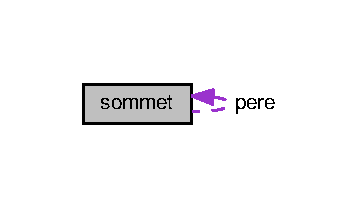
\includegraphics[width=172pt]{structsommet__coll__graph}
\end{center}
\end{figure}
\subsection*{Attributs publics}
\begin{DoxyCompactItemize}
\item 
\hypertarget{structsommet_ae1cd921218c6cb425df68368e1eeef91}{couleur\+\_\+t {\bfseries couleur}}\label{structsommet_ae1cd921218c6cb425df68368e1eeef91}

\item 
\hypertarget{structsommet_ab118367f38ea1cfd0ea0d8c882823ed2}{int {\bfseries f}}\label{structsommet_ab118367f38ea1cfd0ea0d8c882823ed2}

\item 
\hypertarget{structsommet_a95a15dd5bd63851dd9a184881714c970}{int {\bfseries d}}\label{structsommet_a95a15dd5bd63851dd9a184881714c970}

\item 
\hypertarget{structsommet_a0fa328d5d0655b6367bb151f814031fe}{int {\bfseries val}}\label{structsommet_a0fa328d5d0655b6367bb151f814031fe}

\item 
\hypertarget{structsommet_af19efcb82032b6374c1b2c3521c855e1}{struct \hyperlink{structsommet}{sommet} $\ast$ {\bfseries pere}}\label{structsommet_af19efcb82032b6374c1b2c3521c855e1}

\end{DoxyCompactItemize}


\subsection{Description détaillée}


Définition à la ligne 6 du fichier file.\+hpp.



La documentation de cette structure a été générée à partir du fichier suivant \+:\begin{DoxyCompactItemize}
\item 
file.\+hpp\end{DoxyCompactItemize}

\hypertarget{classStructure}{\section{Référence de la classe Structure}
\label{classStructure}\index{Structure@{Structure}}
}


Classe gerant les structures de données chargées dans l'I\+H\+M.  




{\ttfamily \#include $<$structure.\+hpp$>$}



Graphe d'héritage de Structure\+:\nopagebreak
\begin{figure}[H]
\begin{center}
\leavevmode
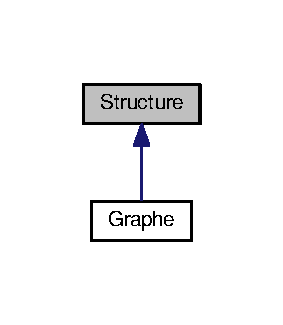
\includegraphics[width=136pt]{classStructure__inherit__graph}
\end{center}
\end{figure}
\subsection*{Fonctions membres publiques}
\begin{DoxyCompactItemize}
\item 
\hyperlink{classStructure_a9d637ea8f6fea642dedfdcdde5947751}{Structure} (std\+::string nom\+\_\+fichier)
\begin{DoxyCompactList}\small\item\em Constructeur de la structure de donnée. \end{DoxyCompactList}\item 
\hypertarget{classStructure_a2d27a247175436df0976f24a83a47b5e}{virtual \hyperlink{classStructure_a2d27a247175436df0976f24a83a47b5e}{$\sim$\+Structure} ()}\label{classStructure_a2d27a247175436df0976f24a83a47b5e}

\begin{DoxyCompactList}\small\item\em Destructeur virtuel. \end{DoxyCompactList}\item 
void \hyperlink{classStructure_a9f9c7f0adff513ccef085b40cee7f6e6}{compute\+\_\+coordonnes} ()
\begin{DoxyCompactList}\small\item\em Calcul du placement. \end{DoxyCompactList}\item 
virtual void \hyperlink{classStructure_ae99db977c0b38122644cf458ea3d5974}{charger} ()=0
\begin{DoxyCompactList}\small\item\em Chargement de la structure de donnée. \end{DoxyCompactList}\item 
bool \hyperlink{classStructure_aa359fa1eec0c2983f10ec94bb14d600b}{est\+\_\+init} ()
\begin{DoxyCompactList}\small\item\em Est initialisé \end{DoxyCompactList}\item 
\hypertarget{classStructure_ad5f67febcbc56fea6c21eb49d43fe028}{std\+::vector$<$ \hyperlink{structSceneVertex}{Scene\+Vertex} $>$ $\ast$ {\bfseries get\+\_\+vertices} ()}\label{classStructure_ad5f67febcbc56fea6c21eb49d43fe028}

\item 
\hypertarget{classStructure_a4157095e5f5cbb1826c5884aac8bba8c}{std\+::vector$<$ G\+Luint $>$ $\ast$ {\bfseries get\+\_\+indices} ()}\label{classStructure_a4157095e5f5cbb1826c5884aac8bba8c}

\end{DoxyCompactItemize}
\subsection*{Attributs protégés}
\begin{DoxyCompactItemize}
\item 
\hypertarget{classStructure_a917ac1b9830c9315200238f8dffd6629}{const char $\ast$ {\bfseries \+\_\+path\+\_\+fichier}}\label{classStructure_a917ac1b9830c9315200238f8dffd6629}

\item 
\hypertarget{classStructure_a47c08f271a4bbbb1ddd1856ea0f4c898}{std\+::vector$<$ \hyperlink{structSceneVertex}{Scene\+Vertex} $>$ {\bfseries \+\_\+vertices}}\label{classStructure_a47c08f271a4bbbb1ddd1856ea0f4c898}

\item 
\hypertarget{classStructure_a1a7966beabdcc5c4c3bf4dae87d566c7}{bool {\bfseries \+\_\+est\+\_\+init}}\label{classStructure_a1a7966beabdcc5c4c3bf4dae87d566c7}

\item 
\hypertarget{classStructure_a32cafffe9f6e0fc75f56c0f45f14528c}{std\+::vector$<$ G\+Luint $>$ {\bfseries \+\_\+indices}}\label{classStructure_a32cafffe9f6e0fc75f56c0f45f14528c}

\end{DoxyCompactItemize}


\subsection{Description détaillée}
Classe gerant les structures de données chargées dans l'I\+H\+M. 

Définition à la ligne 39 du fichier structure.\+hpp.



\subsection{Documentation des constructeurs et destructeur}
\hypertarget{classStructure_a9d637ea8f6fea642dedfdcdde5947751}{\index{Structure@{Structure}!Structure@{Structure}}
\index{Structure@{Structure}!Structure@{Structure}}
\subsubsection[{Structure}]{\setlength{\rightskip}{0pt plus 5cm}Structure\+::\+Structure (
\begin{DoxyParamCaption}
\item[{std\+::string}]{nom\+\_\+fichier}
\end{DoxyParamCaption}
)}}\label{classStructure_a9d637ea8f6fea642dedfdcdde5947751}


Constructeur de la structure de donnée. 

\hyperlink{classStructure}{Structure} de données qui sera chargé de maniere à etre interfaçable dans l'I\+H\+M 
\begin{DoxyParams}[1]{Paramètres}
\mbox{\tt in}  & {\em nom\+\_\+fichier} & nom de fichier à charger pour la structure \\
\hline
\end{DoxyParams}


Définition à la ligne 10 du fichier structure.\+cpp.



\subsection{Documentation des fonctions membres}
\hypertarget{classStructure_ae99db977c0b38122644cf458ea3d5974}{\index{Structure@{Structure}!charger@{charger}}
\index{charger@{charger}!Structure@{Structure}}
\subsubsection[{charger}]{\setlength{\rightskip}{0pt plus 5cm}virtual void Structure\+::charger (
\begin{DoxyParamCaption}
{}
\end{DoxyParamCaption}
)\hspace{0.3cm}{\ttfamily [pure virtual]}}}\label{classStructure_ae99db977c0b38122644cf458ea3d5974}


Chargement de la structure de donnée. 

Chargement de la structure de donnée à partir du fichier, appelé lors de la creation de l'instance courante 
\begin{DoxyParams}[1]{Paramètres}
\mbox{\tt in}  & {\em nom\+\_\+fichier} & nom de fichier qui va etre chargé pour la structure \\
\hline
\end{DoxyParams}


Implémenté dans \hyperlink{classGraphe_a983bd623b721d7485805d252008d82f4}{Graphe}.

\hypertarget{classStructure_a9f9c7f0adff513ccef085b40cee7f6e6}{\index{Structure@{Structure}!compute\+\_\+coordonnes@{compute\+\_\+coordonnes}}
\index{compute\+\_\+coordonnes@{compute\+\_\+coordonnes}!Structure@{Structure}}
\subsubsection[{compute\+\_\+coordonnes}]{\setlength{\rightskip}{0pt plus 5cm}void Structure\+::compute\+\_\+coordonnes (
\begin{DoxyParamCaption}
{}
\end{DoxyParamCaption}
)}}\label{classStructure_a9f9c7f0adff513ccef085b40cee7f6e6}


Calcul du placement. 

Calculer les coordonnées de placement pour l'affichage de la structure de donnée courante 

Définition à la ligne 16 du fichier structure.\+cpp.

\hypertarget{classStructure_aa359fa1eec0c2983f10ec94bb14d600b}{\index{Structure@{Structure}!est\+\_\+init@{est\+\_\+init}}
\index{est\+\_\+init@{est\+\_\+init}!Structure@{Structure}}
\subsubsection[{est\+\_\+init}]{\setlength{\rightskip}{0pt plus 5cm}bool Structure\+::est\+\_\+init (
\begin{DoxyParamCaption}
{}
\end{DoxyParamCaption}
)}}\label{classStructure_aa359fa1eec0c2983f10ec94bb14d600b}


Est initialisé 

permet de savoir si la structure courante est bien initialisé et prete à etre chargé dans la scene opengl 
\begin{DoxyParams}[1]{Paramètres}
\mbox{\tt out}  & {\em retourne} & un booleen specifiant si la structure courante est bien initialisé \\
\hline
\end{DoxyParams}


Définition à la ligne 31 du fichier structure.\+cpp.



La documentation de cette classe a été générée à partir des fichiers suivants \+:\begin{DoxyCompactItemize}
\item 
\hyperlink{structure_8hpp}{structure.\+hpp}\item 
\hyperlink{structure_8cpp}{structure.\+cpp}\end{DoxyCompactItemize}

\hypertarget{classTextBox}{\section{Référence de la classe Text\+Box}
\label{classTextBox}\index{Text\+Box@{Text\+Box}}
}


classe gerant l'affichage de texte durant l'execution  




{\ttfamily \#include $<$textbox.\+hpp$>$}



Graphe d'héritage de Text\+Box\+:\nopagebreak
\begin{figure}[H]
\begin{center}
\leavevmode
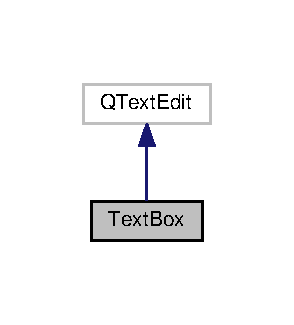
\includegraphics[width=141pt]{classTextBox__inherit__graph}
\end{center}
\end{figure}


Graphe de collaboration de Text\+Box\+:\nopagebreak
\begin{figure}[H]
\begin{center}
\leavevmode
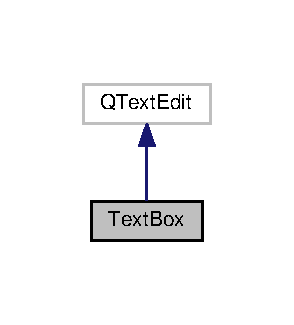
\includegraphics[width=141pt]{classTextBox__coll__graph}
\end{center}
\end{figure}
\subsection*{Fonctions membres publiques}
\begin{DoxyCompactItemize}
\item 
\hyperlink{classTextBox_a8cbbaa2326c8547e180382a58df84243}{Text\+Box} (Q\+Widget $\ast$parent=0)
\begin{DoxyCompactList}\small\item\em Constructeur de la boite de texte. \end{DoxyCompactList}\item 
void \hyperlink{classTextBox_ab124db8fc7720b543a8df13235d6fe96}{afficher} ()
\begin{DoxyCompactList}\small\item\em Met à jour le contenu texte. \end{DoxyCompactList}\item 
void \hyperlink{classTextBox_acca69b10b49ae950a6d2f04c99c7ad80}{ajouter} (std\+::string str, int num\+\_\+ligne)
\begin{DoxyCompactList}\small\item\em Ajoute du texte. \end{DoxyCompactList}\item 
void \hyperlink{classTextBox_a5b4239bff751787a73c0182553822a5f}{remplacer} (std\+::string str, int num\+\_\+ligne, int npos)
\begin{DoxyCompactList}\small\item\em Remplace le texte. \end{DoxyCompactList}\item 
int \hyperlink{classTextBox_a64c57f5a3516613220609a78615df9d0}{newline} ()
\begin{DoxyCompactList}\small\item\em Retourne un numero d'une nouvelle ligne. \end{DoxyCompactList}\item 
\hypertarget{classTextBox_a4c1596312c23884283a8ed1ddc157498}{void \hyperlink{classTextBox_a4c1596312c23884283a8ed1ddc157498}{clear} ()}\label{classTextBox_a4c1596312c23884283a8ed1ddc157498}

\begin{DoxyCompactList}\small\item\em efface le buffer actuel \end{DoxyCompactList}\end{DoxyCompactItemize}


\subsection{Description détaillée}
classe gerant l'affichage de texte durant l'execution 

Définition à la ligne 17 du fichier textbox.\+hpp.



\subsection{Documentation des constructeurs et destructeur}
\hypertarget{classTextBox_a8cbbaa2326c8547e180382a58df84243}{\index{Text\+Box@{Text\+Box}!Text\+Box@{Text\+Box}}
\index{Text\+Box@{Text\+Box}!Text\+Box@{Text\+Box}}
\subsubsection[{Text\+Box}]{\setlength{\rightskip}{0pt plus 5cm}Text\+Box\+::\+Text\+Box (
\begin{DoxyParamCaption}
\item[{Q\+Widget $\ast$}]{parent = {\ttfamily 0}}
\end{DoxyParamCaption}
)}}\label{classTextBox_a8cbbaa2326c8547e180382a58df84243}


Constructeur de la boite de texte. 

il s'agit de text box, on y affichera des informations durant l'execution 
\begin{DoxyParams}[1]{Paramètres}
\mbox{\tt in}  & {\em parent} & le widget parent \\
\hline
\end{DoxyParams}


Définition à la ligne 7 du fichier textbox.\+cpp.



\subsection{Documentation des fonctions membres}
\hypertarget{classTextBox_ab124db8fc7720b543a8df13235d6fe96}{\index{Text\+Box@{Text\+Box}!afficher@{afficher}}
\index{afficher@{afficher}!Text\+Box@{Text\+Box}}
\subsubsection[{afficher}]{\setlength{\rightskip}{0pt plus 5cm}void Text\+Box\+::afficher (
\begin{DoxyParamCaption}
{}
\end{DoxyParamCaption}
)}}\label{classTextBox_ab124db8fc7720b543a8df13235d6fe96}


Met à jour le contenu texte. 

est appelé de manière reguliere par le main thread 

Définition à la ligne 29 du fichier textbox.\+cpp.

\hypertarget{classTextBox_acca69b10b49ae950a6d2f04c99c7ad80}{\index{Text\+Box@{Text\+Box}!ajouter@{ajouter}}
\index{ajouter@{ajouter}!Text\+Box@{Text\+Box}}
\subsubsection[{ajouter}]{\setlength{\rightskip}{0pt plus 5cm}void Text\+Box\+::ajouter (
\begin{DoxyParamCaption}
\item[{std\+::string}]{str, }
\item[{int}]{num\+\_\+ligne}
\end{DoxyParamCaption}
)}}\label{classTextBox_acca69b10b49ae950a6d2f04c99c7ad80}


Ajoute du texte. 

Ajoute du texte à la suite de la ligne 
\begin{DoxyParams}[1]{Paramètres}
\mbox{\tt in}  & {\em str} & texte à ajouter \\
\hline
\mbox{\tt in}  & {\em num\+\_\+ligne} & numero de la ligne \\
\hline
\end{DoxyParams}


Définition à la ligne 51 du fichier textbox.\+cpp.

\hypertarget{classTextBox_a64c57f5a3516613220609a78615df9d0}{\index{Text\+Box@{Text\+Box}!newline@{newline}}
\index{newline@{newline}!Text\+Box@{Text\+Box}}
\subsubsection[{newline}]{\setlength{\rightskip}{0pt plus 5cm}int Text\+Box\+::newline (
\begin{DoxyParamCaption}
{}
\end{DoxyParamCaption}
)}}\label{classTextBox_a64c57f5a3516613220609a78615df9d0}


Retourne un numero d'une nouvelle ligne. 

Permet d'avoir un checkpoint vers une nouvelle ligne pour pouvoir modifier cette ligne grace au numero renvoyé 
\begin{DoxyParams}[1]{Paramètres}
\mbox{\tt out}  & {\em numero} & de ligne \\
\hline
\end{DoxyParams}


Définition à la ligne 63 du fichier textbox.\+cpp.

\hypertarget{classTextBox_a5b4239bff751787a73c0182553822a5f}{\index{Text\+Box@{Text\+Box}!remplacer@{remplacer}}
\index{remplacer@{remplacer}!Text\+Box@{Text\+Box}}
\subsubsection[{remplacer}]{\setlength{\rightskip}{0pt plus 5cm}void Text\+Box\+::remplacer (
\begin{DoxyParamCaption}
\item[{std\+::string}]{str, }
\item[{int}]{num\+\_\+ligne, }
\item[{int}]{npos}
\end{DoxyParamCaption}
)}}\label{classTextBox_a5b4239bff751787a73c0182553822a5f}


Remplace le texte. 

Remplace le texte passé en parametre 
\begin{DoxyParams}[1]{Paramètres}
\mbox{\tt in}  & {\em str} & texte à remplacer \\
\hline
\mbox{\tt in}  & {\em num\+\_\+ligne} & numero de la ligne \\
\hline
\mbox{\tt in}  & {\em npos} & position du premier caractere à remplacer \\
\hline
\end{DoxyParams}


Définition à la ligne 56 du fichier textbox.\+cpp.



La documentation de cette classe a été générée à partir des fichiers suivants \+:\begin{DoxyCompactItemize}
\item 
\hyperlink{textbox_8hpp}{textbox.\+hpp}\item 
\hyperlink{textbox_8cpp}{textbox.\+cpp}\end{DoxyCompactItemize}

\chapter{Documentation des fichiers}
\hypertarget{graphe_8cpp}{\section{Référence du fichier graphe.\+cpp}
\label{graphe_8cpp}\index{graphe.\+cpp@{graphe.\+cpp}}
}


Implementation de \hyperlink{graphe_8hpp}{graphe.\+hpp}.  


{\ttfamily \#include $<$cstdio$>$}\\*
{\ttfamily \#include $<$string$>$}\\*
{\ttfamily \#include \char`\"{}graphe.\+hpp\char`\"{}}\\*
{\ttfamily \#include \char`\"{}file.\+hpp\char`\"{}}\\*
Graphe des dépendances par inclusion de graphe.\+cpp\+:\nopagebreak
\begin{figure}[H]
\begin{center}
\leavevmode
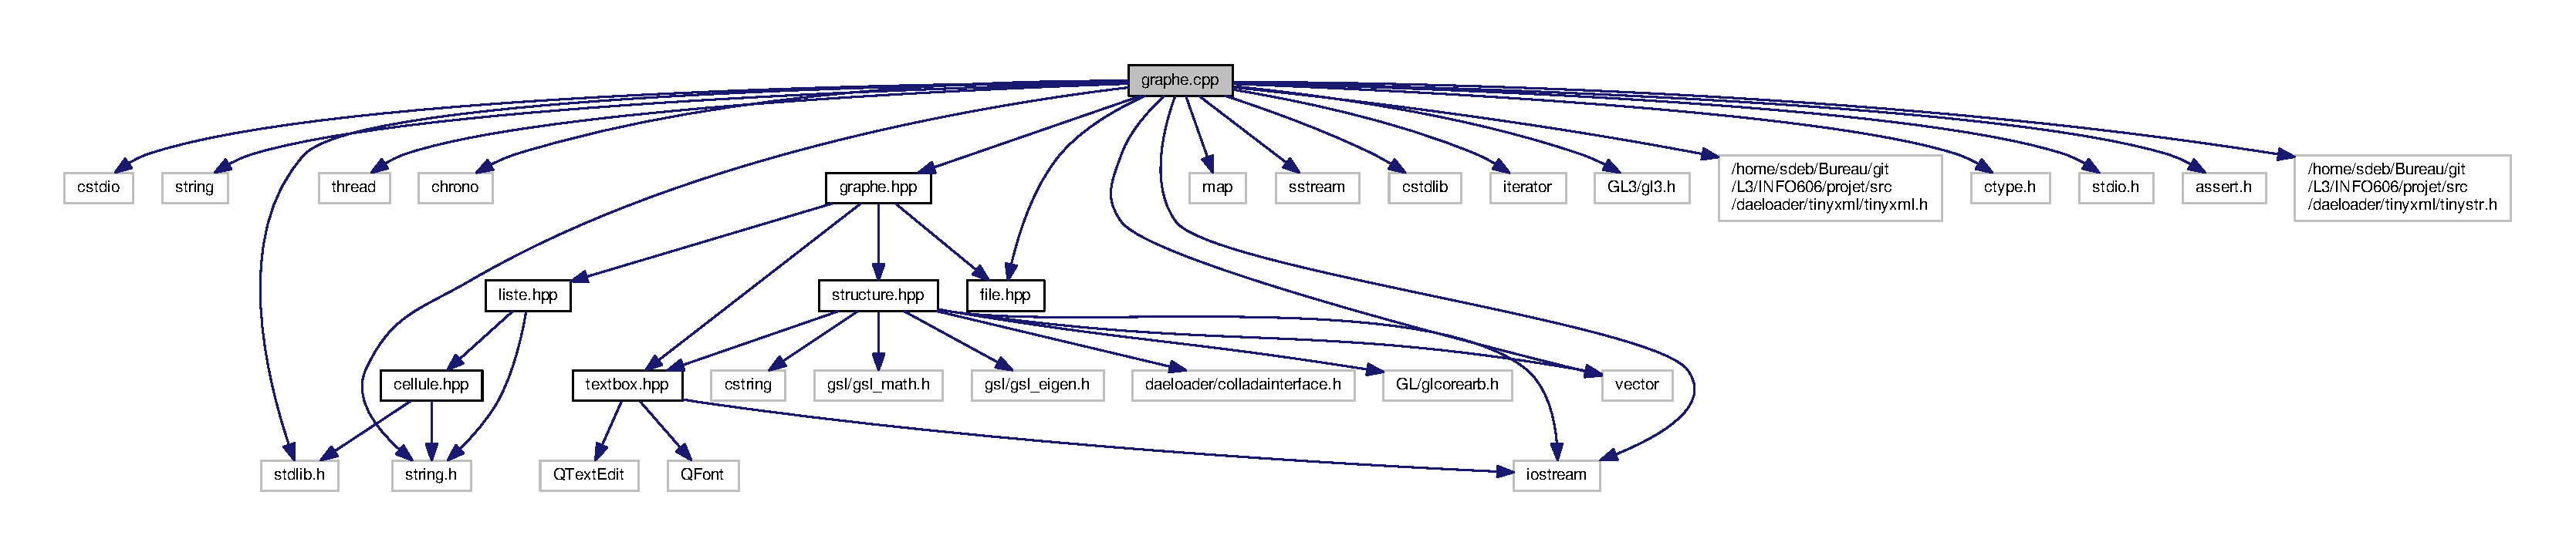
\includegraphics[width=350pt]{graphe_8cpp__incl}
\end{center}
\end{figure}


\subsection{Description détaillée}
Implementation de \hyperlink{graphe_8hpp}{graphe.\+hpp}. 



Définition dans le fichier \hyperlink{graphe_8cpp_source}{graphe.\+cpp}.


\hypertarget{graphe_8hpp}{\section{Référence du fichier graphe.\+hpp}
\label{graphe_8hpp}\index{graphe.\+hpp@{graphe.\+hpp}}
}


Gère la structure de donnée de graphe.  


{\ttfamily \#include \char`\"{}liste.\+hpp\char`\"{}}\\*
{\ttfamily \#include \char`\"{}file.\+hpp\char`\"{}}\\*
{\ttfamily \#include \char`\"{}structure.\+hpp\char`\"{}}\\*
{\ttfamily \#include \char`\"{}textbox.\+hpp\char`\"{}}\\*
Graphe des dépendances par inclusion de graphe.\+hpp\+:\nopagebreak
\begin{figure}[H]
\begin{center}
\leavevmode
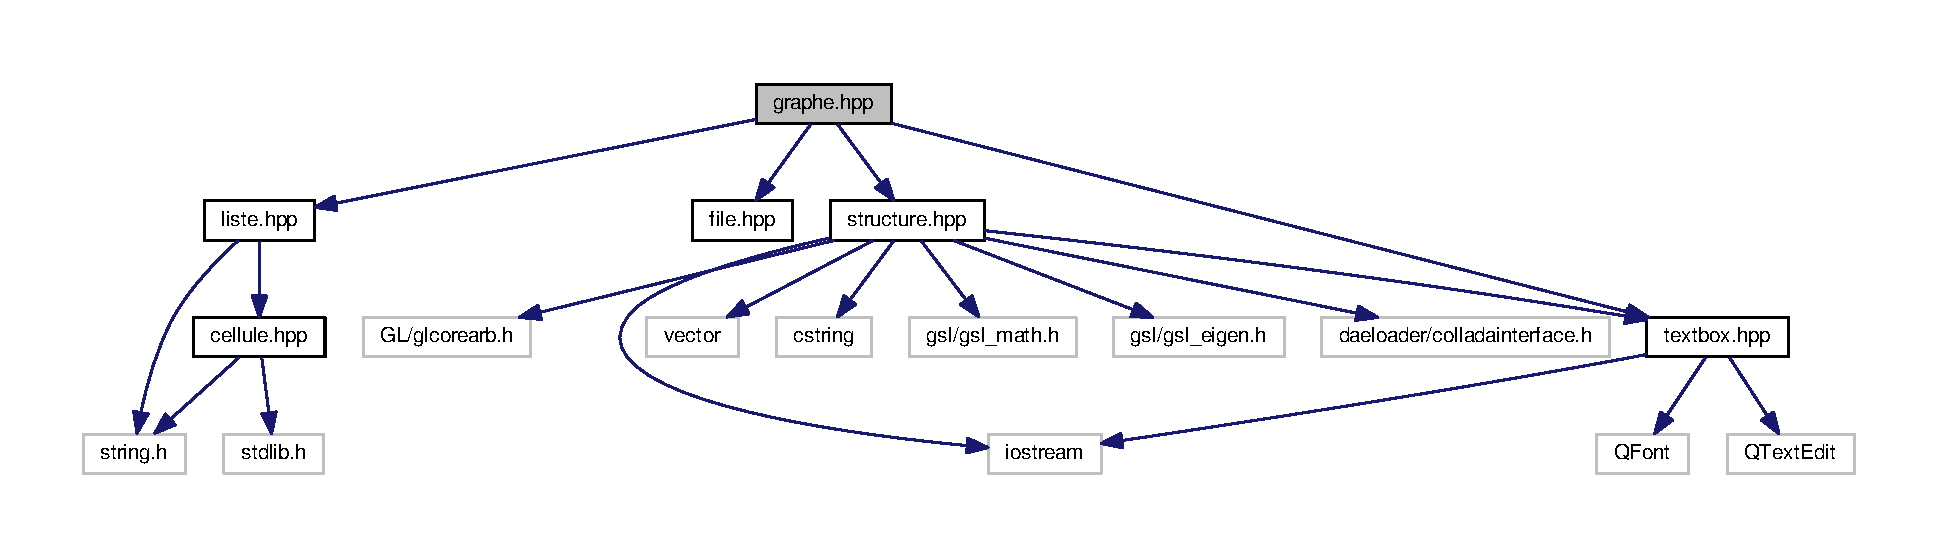
\includegraphics[width=350pt]{graphe_8hpp__incl}
\end{center}
\end{figure}
Ce graphe montre quels fichiers incluent directement ou indirectement ce fichier \+:\nopagebreak
\begin{figure}[H]
\begin{center}
\leavevmode
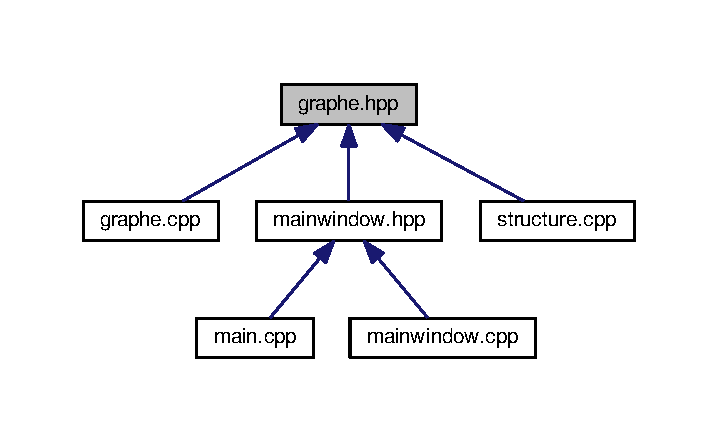
\includegraphics[width=345pt]{graphe_8hpp__dep__incl}
\end{center}
\end{figure}
\subsection*{Classes}
\begin{DoxyCompactItemize}
\item 
struct \hyperlink{structliste__adjacence__t}{liste\+\_\+adjacence\+\_\+t}
\item 
struct \hyperlink{structmatrice__laplace__t}{matrice\+\_\+laplace\+\_\+t}
\item 
struct \hyperlink{structmatrice__adjacence__t}{matrice\+\_\+adjacence\+\_\+t}
\item 
struct \hyperlink{structparcours__t}{parcours\+\_\+t}
\item 
class \hyperlink{classGraphe}{Graphe}
\begin{DoxyCompactList}\small\item\em Classe gerant la structure de donnée de graphe. \end{DoxyCompactList}\end{DoxyCompactItemize}


\subsection{Description détaillée}
Gère la structure de donnée de graphe. 



Définition dans le fichier \hyperlink{graphe_8hpp_source}{graphe.\+hpp}.


\hypertarget{main_8cpp}{\section{Référence du fichier main.\+cpp}
\label{main_8cpp}\index{main.\+cpp@{main.\+cpp}}
}


Programme principale.  


{\ttfamily \#include $<$Q\+Application$>$}\\*
{\ttfamily \#include $<$Q\+Set$>$}\\*
{\ttfamily \#include $<$Q\+File$>$}\\*
{\ttfamily \#include $<$Q\+File\+System\+Watcher$>$}\\*
{\ttfamily \#include $<$vector$>$}\\*
{\ttfamily \#include \char`\"{}mainwindow.\+hpp\char`\"{}}\\*
Graphe des dépendances par inclusion de main.\+cpp\+:\nopagebreak
\begin{figure}[H]
\begin{center}
\leavevmode
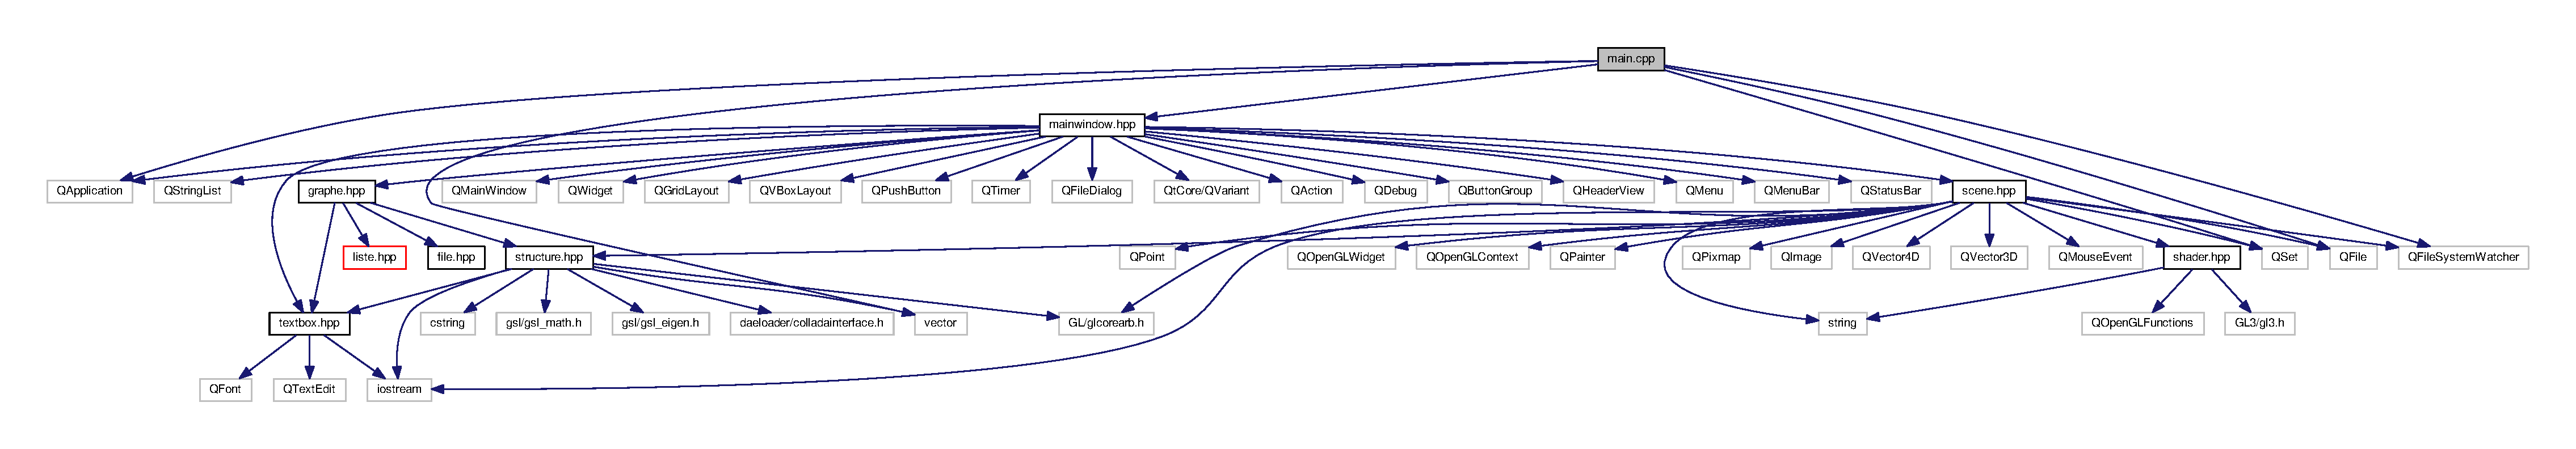
\includegraphics[width=350pt]{main_8cpp__incl}
\end{center}
\end{figure}
\subsection*{Fonctions}
\begin{DoxyCompactItemize}
\item 
\hypertarget{main_8cpp_a0ddf1224851353fc92bfbff6f499fa97}{int {\bfseries main} (int argc, char $\ast$argv\mbox{[}$\,$\mbox{]})}\label{main_8cpp_a0ddf1224851353fc92bfbff6f499fa97}

\end{DoxyCompactItemize}


\subsection{Description détaillée}
Programme principale. 



Définition dans le fichier \hyperlink{main_8cpp_source}{main.\+cpp}.


\hypertarget{mainwindow_8cpp}{\section{Référence du fichier mainwindow.\+cpp}
\label{mainwindow_8cpp}\index{mainwindow.\+cpp@{mainwindow.\+cpp}}
}


Implementation de \hyperlink{mainwindow_8hpp}{mainwindow.\+hpp}.  


{\ttfamily \#include \char`\"{}mainwindow.\+hpp\char`\"{}}\\*
Graphe des dépendances par inclusion de mainwindow.\+cpp\+:\nopagebreak
\begin{figure}[H]
\begin{center}
\leavevmode
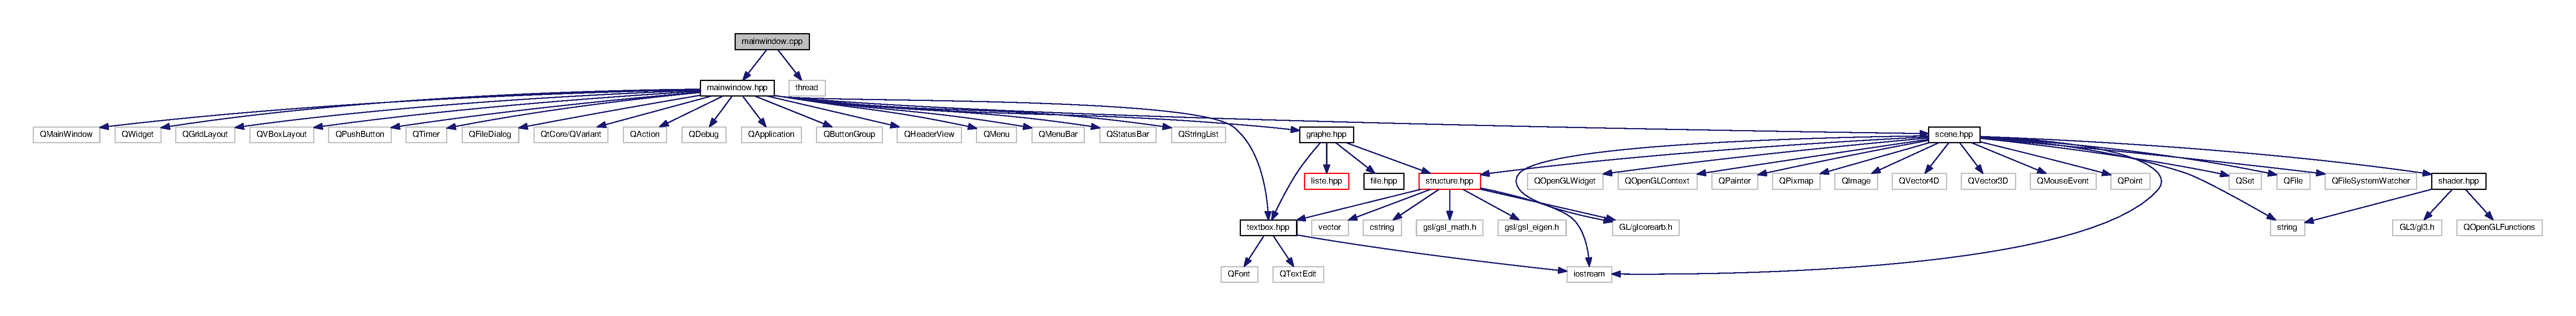
\includegraphics[width=350pt]{mainwindow_8cpp__incl}
\end{center}
\end{figure}


\subsection{Description détaillée}
Implementation de \hyperlink{mainwindow_8hpp}{mainwindow.\+hpp}. 



Définition dans le fichier \hyperlink{mainwindow_8cpp_source}{mainwindow.\+cpp}.


\hypertarget{mainwindow_8hpp}{\section{Référence du fichier mainwindow.\+hpp}
\label{mainwindow_8hpp}\index{mainwindow.\+hpp@{mainwindow.\+hpp}}
}


Gère la fenetre principale.  


{\ttfamily \#include $<$Q\+Main\+Window$>$}\\*
{\ttfamily \#include $<$Q\+Widget$>$}\\*
{\ttfamily \#include $<$Q\+Grid\+Layout$>$}\\*
{\ttfamily \#include $<$Q\+V\+Box\+Layout$>$}\\*
{\ttfamily \#include $<$Q\+Push\+Button$>$}\\*
{\ttfamily \#include $<$Q\+Timer$>$}\\*
{\ttfamily \#include $<$Q\+File\+Dialog$>$}\\*
{\ttfamily \#include $<$Qt\+Core/\+Q\+Variant$>$}\\*
{\ttfamily \#include $<$Q\+Action$>$}\\*
{\ttfamily \#include $<$Q\+Debug$>$}\\*
{\ttfamily \#include $<$Q\+Application$>$}\\*
{\ttfamily \#include $<$Q\+Button\+Group$>$}\\*
{\ttfamily \#include $<$Q\+Header\+View$>$}\\*
{\ttfamily \#include $<$Q\+Menu$>$}\\*
{\ttfamily \#include $<$Q\+Menu\+Bar$>$}\\*
{\ttfamily \#include $<$Q\+Status\+Bar$>$}\\*
{\ttfamily \#include $<$Q\+String\+List$>$}\\*
{\ttfamily \#include \char`\"{}textbox.\+hpp\char`\"{}}\\*
{\ttfamily \#include \char`\"{}scene.\+hpp\char`\"{}}\\*
{\ttfamily \#include \char`\"{}graphe.\+hpp\char`\"{}}\\*
Graphe des dépendances par inclusion de mainwindow.\+hpp\+:\nopagebreak
\begin{figure}[H]
\begin{center}
\leavevmode
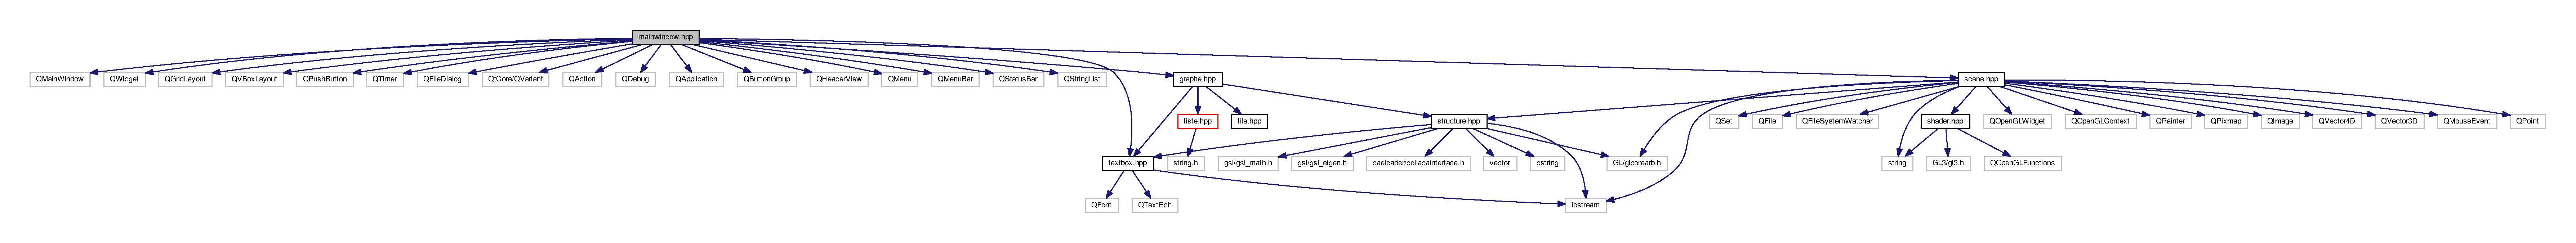
\includegraphics[width=350pt]{mainwindow_8hpp__incl}
\end{center}
\end{figure}
Ce graphe montre quels fichiers incluent directement ou indirectement ce fichier \+:\nopagebreak
\begin{figure}[H]
\begin{center}
\leavevmode
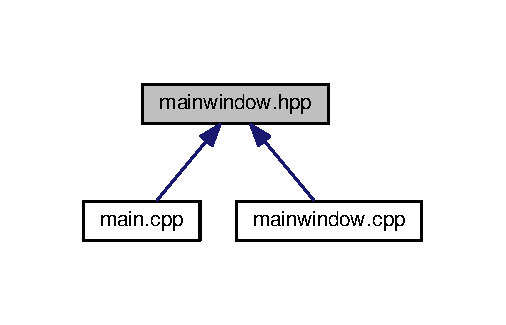
\includegraphics[width=243pt]{mainwindow_8hpp__dep__incl}
\end{center}
\end{figure}
\subsection*{Classes}
\begin{DoxyCompactItemize}
\item 
class \hyperlink{classMainWindow}{Main\+Window}
\begin{DoxyCompactList}\small\item\em classe gerant le placement et interactions des principaux widgets dans la fenetre principale \end{DoxyCompactList}\end{DoxyCompactItemize}


\subsection{Description détaillée}
Gère la fenetre principale. 



Définition dans le fichier \hyperlink{mainwindow_8hpp_source}{mainwindow.\+hpp}.


\hypertarget{scene_8cpp}{\section{Référence du fichier scene.\+cpp}
\label{scene_8cpp}\index{scene.\+cpp@{scene.\+cpp}}
}


Implementation de \hyperlink{scene_8hpp}{scene.\+hpp}.  


{\ttfamily \#include $<$glm/glm.\+hpp$>$}\\*
{\ttfamily \#include $<$glm/gtx/transform.\+hpp$>$}\\*
{\ttfamily \#include $<$glm/gtc/type\+\_\+ptr.\+hpp$>$}\\*
{\ttfamily \#include $<$iostream$>$}\\*
{\ttfamily \#include $<$string$>$}\\*
{\ttfamily \#include $<$functional$>$}\\*
{\ttfamily \#include \char`\"{}scene.\+hpp\char`\"{}}\\*
Graphe des dépendances par inclusion de scene.\+cpp\+:\nopagebreak
\begin{figure}[H]
\begin{center}
\leavevmode
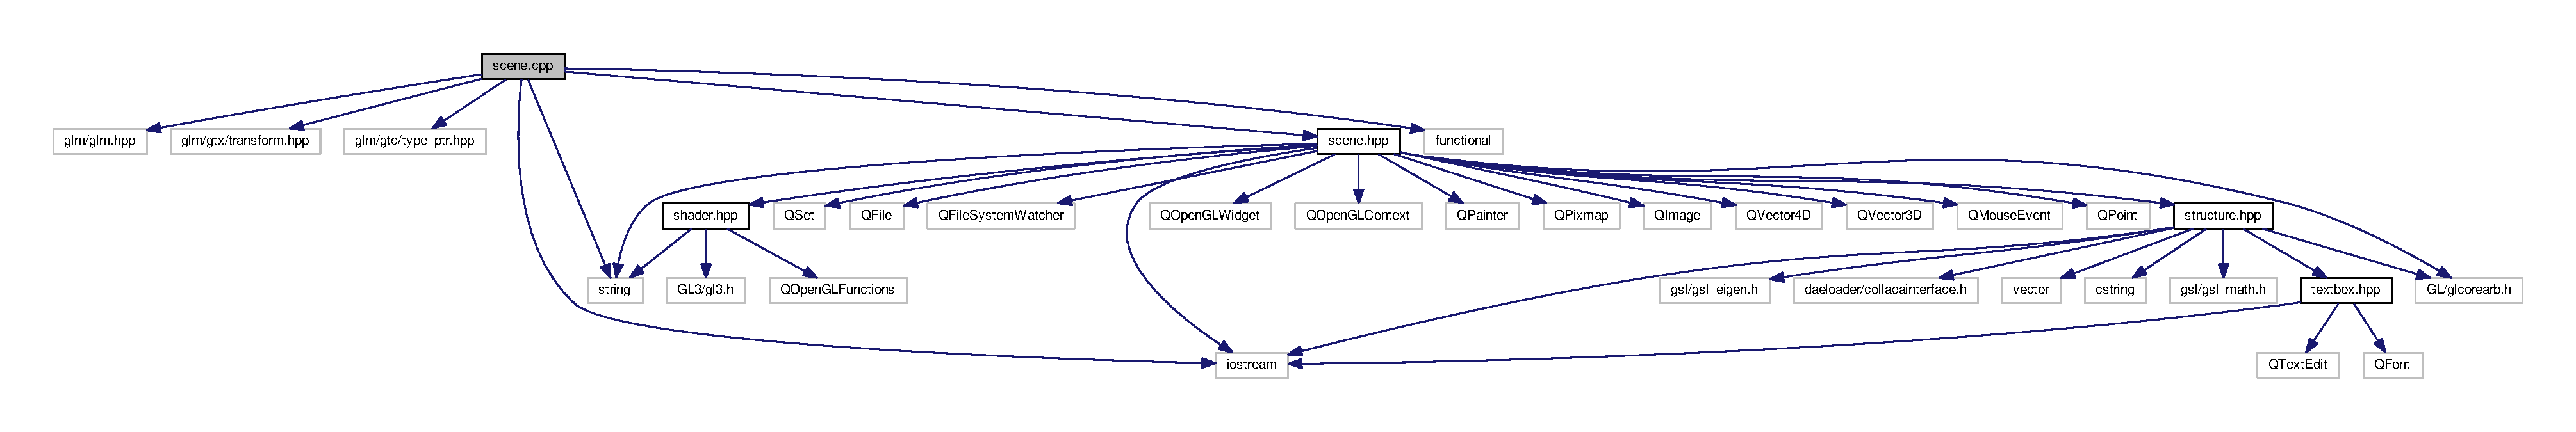
\includegraphics[width=350pt]{scene_8cpp__incl}
\end{center}
\end{figure}
\subsection*{Classes}
\begin{DoxyCompactItemize}
\item 
struct \hyperlink{structparam__lux}{param\+\_\+lux}
\end{DoxyCompactItemize}
\subsection*{Macros}
\begin{DoxyCompactItemize}
\item 
\hypertarget{scene_8cpp_a816ab7d5c2ce1f0a01216042837beb93}{\#define {\bfseries G\+L\+M\+\_\+\+F\+O\+R\+C\+E\+\_\+\+R\+A\+D\+I\+A\+N\+S}}\label{scene_8cpp_a816ab7d5c2ce1f0a01216042837beb93}

\item 
\hypertarget{scene_8cpp_ac7b3a9f069bf13fef2ece8337f933fb5}{\#define {\bfseries A\+F\+F\+D\+E\+B\+U\+G}~1}\label{scene_8cpp_ac7b3a9f069bf13fef2ece8337f933fb5}

\item 
\#define {\bfseries W\+A\+R\+N}(M\+S\+G)
\item 
\#define {\bfseries I\+S\+O\+K}(M\+S\+G)
\end{DoxyCompactItemize}
\subsection*{Variables}
\begin{DoxyCompactItemize}
\item 
\hypertarget{scene_8cpp_a5f18c7186cd8bb18342e1294505fa63c}{double {\bfseries angle\+Y} = 0.\+0}\label{scene_8cpp_a5f18c7186cd8bb18342e1294505fa63c}

\item 
\hypertarget{scene_8cpp_aa834f0cff99511d8ba9b1c04bdea07eb}{double {\bfseries angle\+Z} = 0.\+0}\label{scene_8cpp_aa834f0cff99511d8ba9b1c04bdea07eb}

\item 
\hypertarget{scene_8cpp_add1bbbe708372f7d961669f4520ecaa7}{int {\bfseries old\+\_\+posx} = 0}\label{scene_8cpp_add1bbbe708372f7d961669f4520ecaa7}

\item 
\hypertarget{scene_8cpp_aa818cdb551875a5ba4b87c157167e488}{int {\bfseries old\+\_\+posy} = 0}\label{scene_8cpp_aa818cdb551875a5ba4b87c157167e488}

\item 
\hypertarget{scene_8cpp_abdac33eeb786cfd354032f8e94c27070}{bool {\bfseries \+\_\+hold} = false}\label{scene_8cpp_abdac33eeb786cfd354032f8e94c27070}

\end{DoxyCompactItemize}


\subsection{Description détaillée}
Implementation de \hyperlink{scene_8hpp}{scene.\+hpp}. 



Définition dans le fichier \hyperlink{scene_8cpp_source}{scene.\+cpp}.



\subsection{Documentation des macros}
\hypertarget{scene_8cpp_ac8055c7eae91b1c50a3189f735c54c73}{\index{scene.\+cpp@{scene.\+cpp}!I\+S\+O\+K@{I\+S\+O\+K}}
\index{I\+S\+O\+K@{I\+S\+O\+K}!scene.\+cpp@{scene.\+cpp}}
\subsubsection[{I\+S\+O\+K}]{\setlength{\rightskip}{0pt plus 5cm}\#define I\+S\+O\+K(
\begin{DoxyParamCaption}
\item[{}]{M\+S\+G}
\end{DoxyParamCaption}
)}}\label{scene_8cpp_ac8055c7eae91b1c50a3189f735c54c73}
{\bfseries Valeur \+:}
\begin{DoxyCode}
printf(\textcolor{stringliteral}{"\(\backslash\)n\(\backslash\)033[42;01m"}                                \(\backslash\)
                         \textcolor{stringliteral}{"[\_POSITION\_]\(\backslash\)t[%s:%d] -> [%s]\(\backslash\)n"}              \(\backslash\)
                         \textcolor{stringliteral}{"[\_DEBUG\_MSG\_]\(\backslash\)t[%s]"}                          \(\backslash\)
                         \textcolor{stringliteral}{"\(\backslash\)033[00m\(\backslash\)n"}, \_\_FILE\_\_, \_\_LINE\_\_, \_\_func\_\_, MSG);
\end{DoxyCode}


Définition à la ligne 36 du fichier scene.\+cpp.

\hypertarget{scene_8cpp_a54c0b0a398d16827eb0609c67d519af0}{\index{scene.\+cpp@{scene.\+cpp}!W\+A\+R\+N@{W\+A\+R\+N}}
\index{W\+A\+R\+N@{W\+A\+R\+N}!scene.\+cpp@{scene.\+cpp}}
\subsubsection[{W\+A\+R\+N}]{\setlength{\rightskip}{0pt plus 5cm}\#define W\+A\+R\+N(
\begin{DoxyParamCaption}
\item[{}]{M\+S\+G}
\end{DoxyParamCaption}
)}}\label{scene_8cpp_a54c0b0a398d16827eb0609c67d519af0}
{\bfseries Valeur \+:}
\begin{DoxyCode}
printf(\textcolor{stringliteral}{"\(\backslash\)n\(\backslash\)033[41;01m"}                                \(\backslash\)
                         \textcolor{stringliteral}{"[\_POSITION\_]\(\backslash\)t[%s:%d] -> [%s]\(\backslash\)n"}              \(\backslash\)
                         \textcolor{stringliteral}{"[\_DEBUG\_MSG\_]\(\backslash\)t[%s]"}                          \(\backslash\)
                         \textcolor{stringliteral}{"\(\backslash\)033[00m\(\backslash\)n"}, \_\_FILE\_\_, \_\_LINE\_\_, \_\_func\_\_, MSG);
\end{DoxyCode}


Définition à la ligne 31 du fichier scene.\+cpp.


\hypertarget{scene_8hpp}{\section{Référence du fichier scene.\+hpp}
\label{scene_8hpp}\index{scene.\+hpp@{scene.\+hpp}}
}


Gère le contexte Open\+G\+L.  


{\ttfamily \#include $<$Q\+Set$>$}\\*
{\ttfamily \#include $<$Q\+File$>$}\\*
{\ttfamily \#include $<$Q\+File\+System\+Watcher$>$}\\*
{\ttfamily \#include $<$G\+L/glcorearb.\+h$>$}\\*
{\ttfamily \#include $<$Q\+Open\+G\+L\+Widget$>$}\\*
{\ttfamily \#include $<$Q\+Open\+G\+L\+Context$>$}\\*
{\ttfamily \#include $<$Q\+Painter$>$}\\*
{\ttfamily \#include $<$Q\+Pixmap$>$}\\*
{\ttfamily \#include $<$Q\+Image$>$}\\*
{\ttfamily \#include $<$Q\+Vector4\+D$>$}\\*
{\ttfamily \#include $<$Q\+Vector3\+D$>$}\\*
{\ttfamily \#include $<$Q\+Mouse\+Event$>$}\\*
{\ttfamily \#include $<$Q\+Point$>$}\\*
{\ttfamily \#include $<$iostream$>$}\\*
{\ttfamily \#include $<$string$>$}\\*
{\ttfamily \#include \char`\"{}shader.\+hpp\char`\"{}}\\*
{\ttfamily \#include \char`\"{}structure.\+hpp\char`\"{}}\\*
Graphe des dépendances par inclusion de scene.\+hpp\+:\nopagebreak
\begin{figure}[H]
\begin{center}
\leavevmode
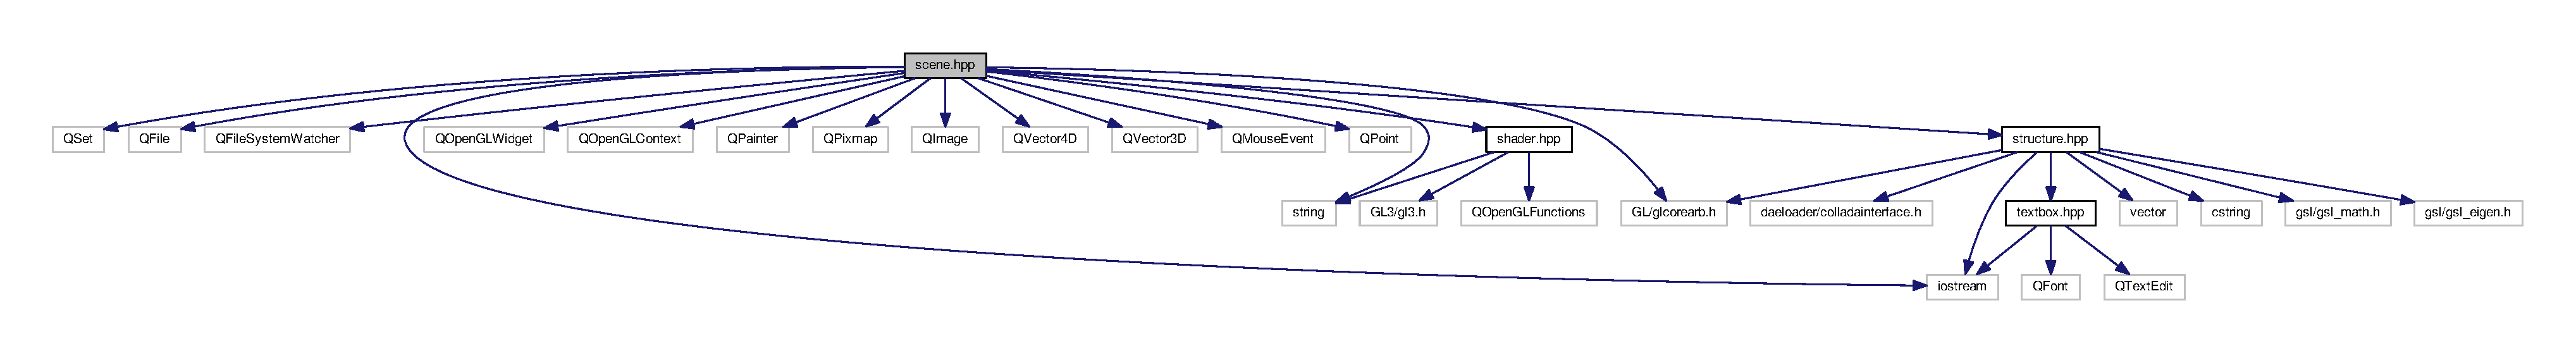
\includegraphics[width=350pt]{scene_8hpp__incl}
\end{center}
\end{figure}
Ce graphe montre quels fichiers incluent directement ou indirectement ce fichier \+:\nopagebreak
\begin{figure}[H]
\begin{center}
\leavevmode
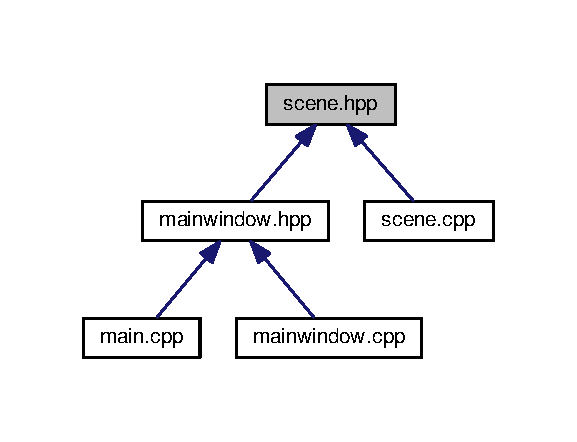
\includegraphics[width=277pt]{scene_8hpp__dep__incl}
\end{center}
\end{figure}
\subsection*{Classes}
\begin{DoxyCompactItemize}
\item 
struct \hyperlink{structDataNode}{Data\+Node}
\item 
class \hyperlink{classSceneGL}{Scene\+G\+L}
\begin{DoxyCompactList}\small\item\em classe gerant le contexte Open\+G\+L de l'application \end{DoxyCompactList}\end{DoxyCompactItemize}


\subsection{Description détaillée}
Gère le contexte Open\+G\+L. 



Définition dans le fichier \hyperlink{scene_8hpp_source}{scene.\+hpp}.


\hypertarget{shader_8cpp}{\section{Référence du fichier shader.\+cpp}
\label{shader_8cpp}\index{shader.\+cpp@{shader.\+cpp}}
}


Implementation de \hyperlink{shader_8hpp}{shader.\+hpp}.  


{\ttfamily \#include $<$iostream$>$}\\*
{\ttfamily \#include $<$fstream$>$}\\*
{\ttfamily \#include \char`\"{}shader.\+hpp\char`\"{}}\\*
Graphe des dépendances par inclusion de shader.\+cpp\+:\nopagebreak
\begin{figure}[H]
\begin{center}
\leavevmode
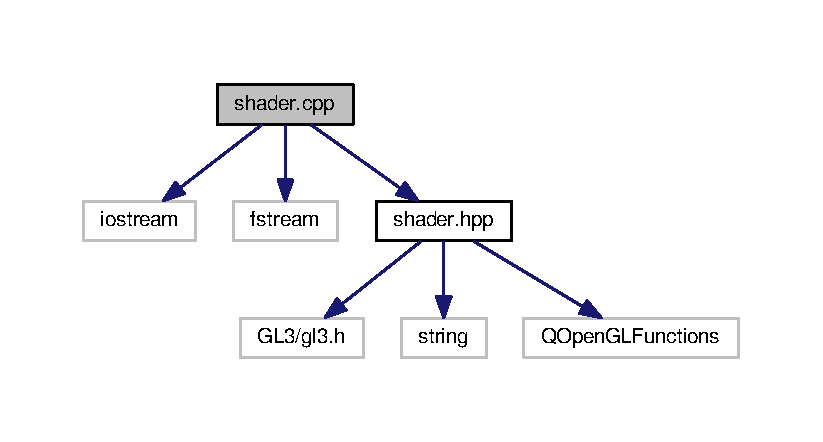
\includegraphics[width=350pt]{shader_8cpp__incl}
\end{center}
\end{figure}


\subsection{Description détaillée}
Implementation de \hyperlink{shader_8hpp}{shader.\+hpp}. 



Définition dans le fichier \hyperlink{shader_8cpp_source}{shader.\+cpp}.


\hypertarget{shader_8hpp}{\section{Référence du fichier shader.\+hpp}
\label{shader_8hpp}\index{shader.\+hpp@{shader.\+hpp}}
}


Gère les shaders.  


{\ttfamily \#include $<$G\+L3/gl3.\+h$>$}\\*
{\ttfamily \#include $<$string$>$}\\*
{\ttfamily \#include $<$Q\+Open\+G\+L\+Functions$>$}\\*
Graphe des dépendances par inclusion de shader.\+hpp\+:\nopagebreak
\begin{figure}[H]
\begin{center}
\leavevmode
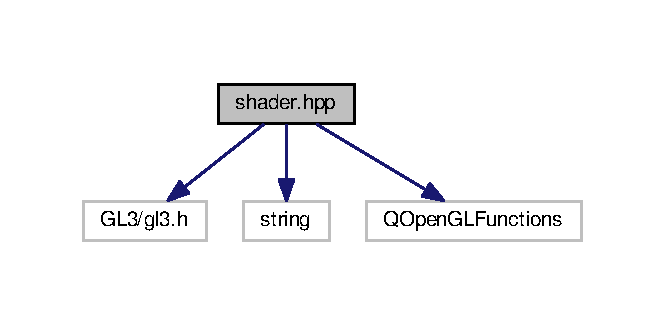
\includegraphics[width=319pt]{shader_8hpp__incl}
\end{center}
\end{figure}
Ce graphe montre quels fichiers incluent directement ou indirectement ce fichier \+:\nopagebreak
\begin{figure}[H]
\begin{center}
\leavevmode
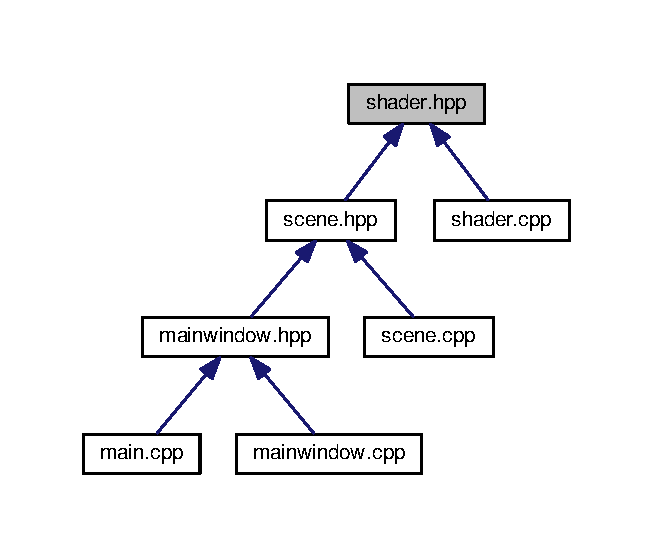
\includegraphics[width=314pt]{shader_8hpp__dep__incl}
\end{center}
\end{figure}
\subsection*{Classes}
\begin{DoxyCompactItemize}
\item 
class \hyperlink{classShader}{Shader}
\begin{DoxyCompactList}\small\item\em Classe gerant la compilation et verrouillage du vertex et fragment shaders. \end{DoxyCompactList}\end{DoxyCompactItemize}
\subsection*{Macros}
\begin{DoxyCompactItemize}
\item 
\hypertarget{shader_8hpp_a513ae87770898727d346eced6be03bdd}{\#define {\bfseries G\+L3\+\_\+\+P\+R\+O\+T\+O\+T\+Y\+P\+E\+S}~1}\label{shader_8hpp_a513ae87770898727d346eced6be03bdd}

\end{DoxyCompactItemize}


\subsection{Description détaillée}
Gère les shaders. 



Définition dans le fichier \hyperlink{shader_8hpp_source}{shader.\+hpp}.


\hypertarget{structure_8cpp}{\section{Référence du fichier structure.\+cpp}
\label{structure_8cpp}\index{structure.\+cpp@{structure.\+cpp}}
}


Implementation de \hyperlink{structure_8hpp}{structure.\+hpp}.  


{\ttfamily \#include \char`\"{}graphe.\+hpp\char`\"{}}\\*
{\ttfamily \#include \char`\"{}structure.\+hpp\char`\"{}}\\*
Graphe des dépendances par inclusion de structure.\+cpp\+:\nopagebreak
\begin{figure}[H]
\begin{center}
\leavevmode
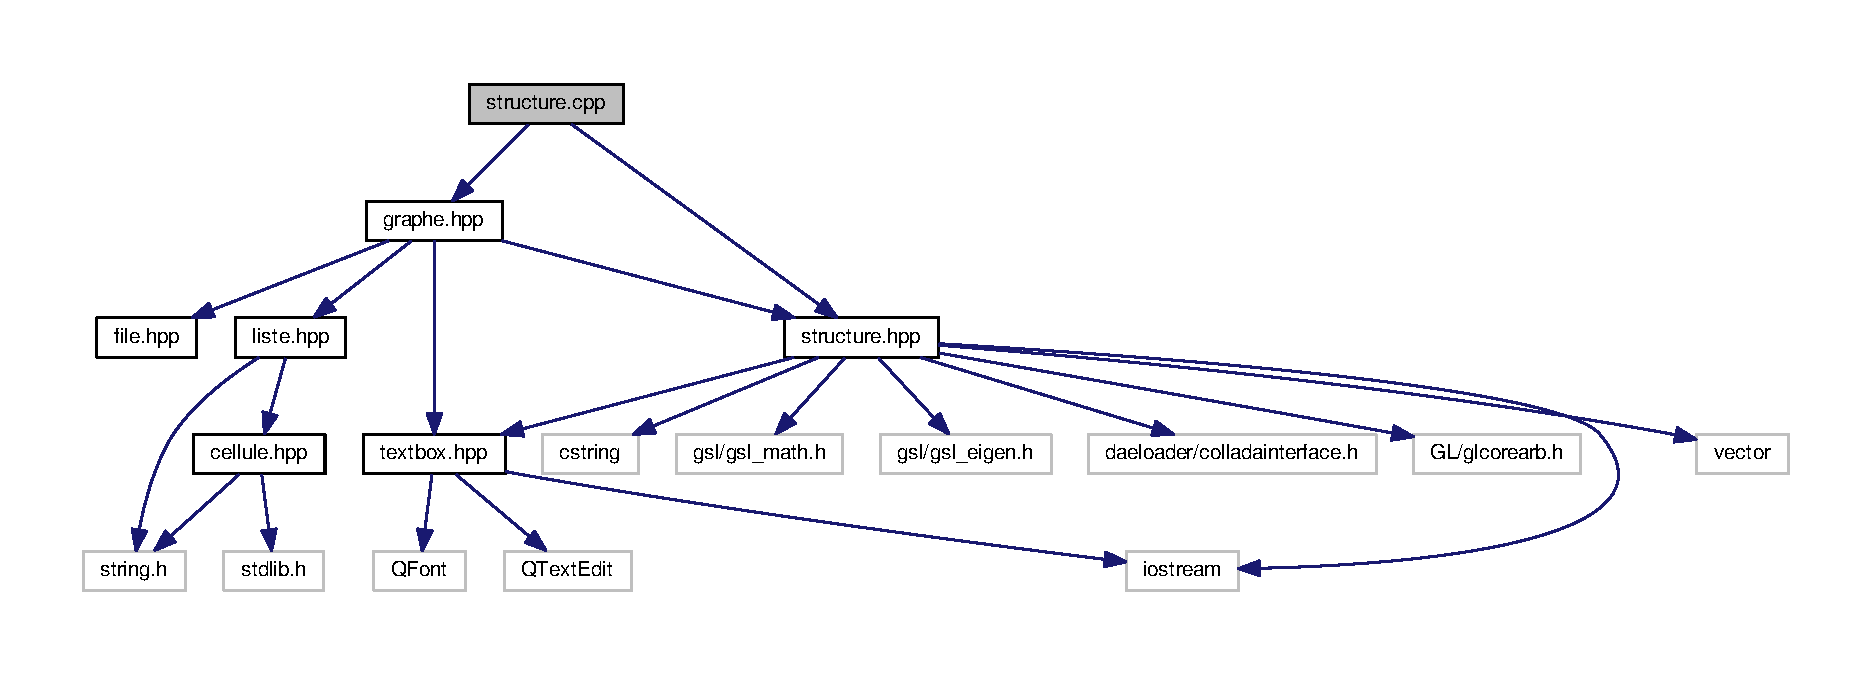
\includegraphics[width=350pt]{structure_8cpp__incl}
\end{center}
\end{figure}


\subsection{Description détaillée}
Implementation de \hyperlink{structure_8hpp}{structure.\+hpp}. 



Définition dans le fichier \hyperlink{structure_8cpp_source}{structure.\+cpp}.


\hypertarget{structure_8hpp}{\section{Référence du fichier structure.\+hpp}
\label{structure_8hpp}\index{structure.\+hpp@{structure.\+hpp}}
}


Gère les structures de données.  


{\ttfamily \#include $<$G\+L/glcorearb.\+h$>$}\\*
{\ttfamily \#include $<$iostream$>$}\\*
{\ttfamily \#include $<$vector$>$}\\*
{\ttfamily \#include $<$cstring$>$}\\*
{\ttfamily \#include $<$gsl/gsl\+\_\+math.\+h$>$}\\*
{\ttfamily \#include $<$gsl/gsl\+\_\+eigen.\+h$>$}\\*
{\ttfamily \#include \char`\"{}daeloader/colladainterface.\+h\char`\"{}}\\*
{\ttfamily \#include \char`\"{}textbox.\+hpp\char`\"{}}\\*
Graphe des dépendances par inclusion de structure.\+hpp\+:\nopagebreak
\begin{figure}[H]
\begin{center}
\leavevmode
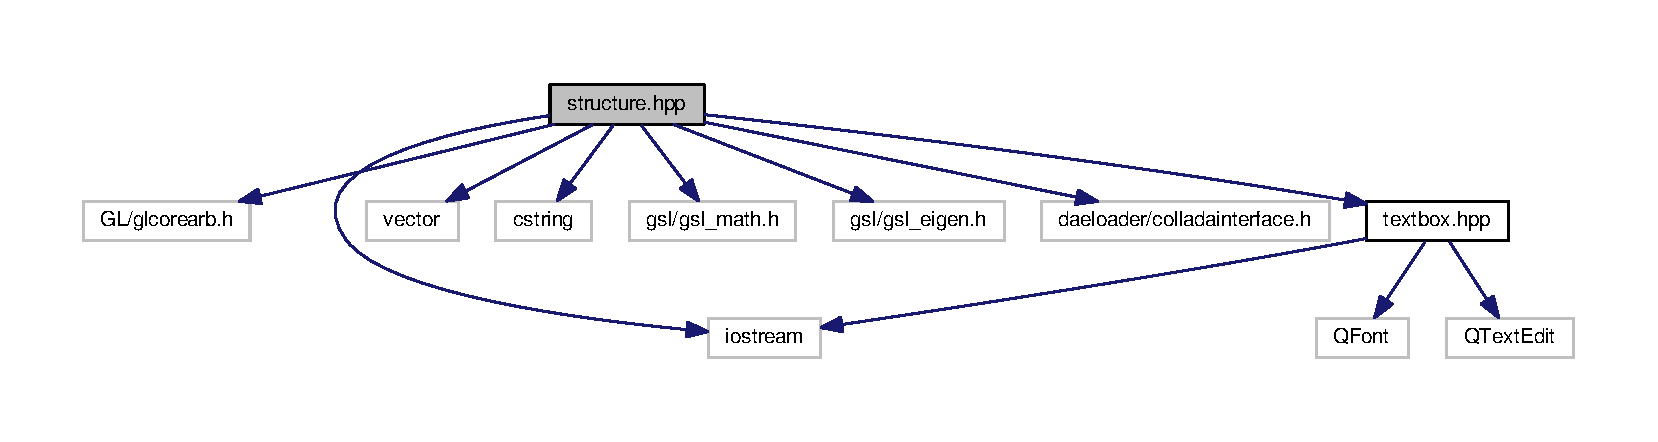
\includegraphics[width=350pt]{structure_8hpp__incl}
\end{center}
\end{figure}
Ce graphe montre quels fichiers incluent directement ou indirectement ce fichier \+:\nopagebreak
\begin{figure}[H]
\begin{center}
\leavevmode
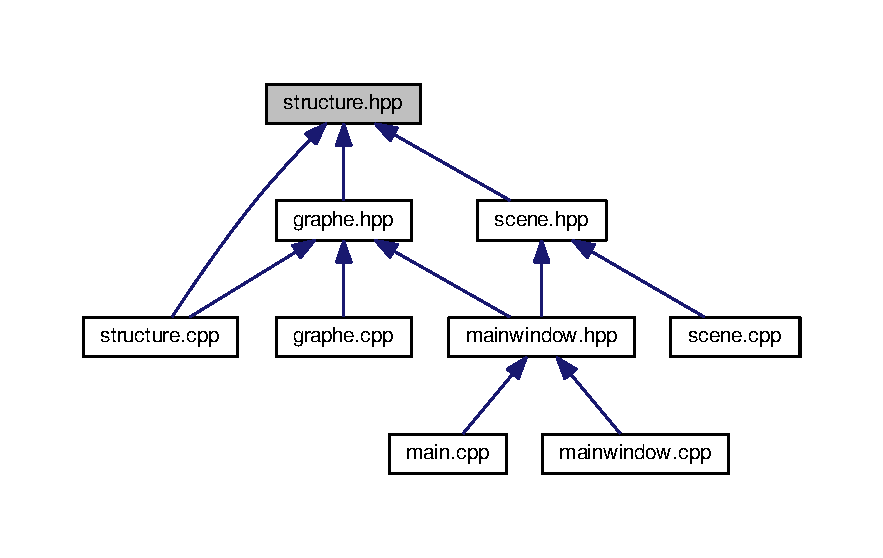
\includegraphics[width=350pt]{structure_8hpp__dep__incl}
\end{center}
\end{figure}
\subsection*{Classes}
\begin{DoxyCompactItemize}
\item 
struct \hyperlink{structSceneVertex}{Scene\+Vertex}
\begin{DoxyCompactList}\small\item\em structure d'un vertex incluant sa position et couleur \end{DoxyCompactList}\item 
class \hyperlink{classStructure}{Structure}
\begin{DoxyCompactList}\small\item\em Classe gerant les structures de données chargées dans l'I\+H\+M. \end{DoxyCompactList}\end{DoxyCompactItemize}
\subsection*{Énumérations}
\begin{DoxyCompactItemize}
\item 
\hypertarget{namespaceEtat_a9067ede406d5ecdd73ca17421b0119ca}{enum {\bfseries Noeud} \{ \\*
{\bfseries S\+I\+M\+P\+L\+E}, 
{\bfseries C\+O\+U\+R\+A\+N\+T}, 
{\bfseries V\+I\+S\+I\+T\+E\+D}, 
{\bfseries S\+E\+L\+E\+C\+T}, 
\\*
{\bfseries C\+H\+O\+I\+X}
 \}}\label{namespaceEtat_a9067ede406d5ecdd73ca17421b0119ca}

\end{DoxyCompactItemize}


\subsection{Description détaillée}
Gère les structures de données. 



Définition dans le fichier \hyperlink{structure_8hpp_source}{structure.\+hpp}.


\hypertarget{textbox_8cpp}{\section{Référence du fichier textbox.\+cpp}
\label{textbox_8cpp}\index{textbox.\+cpp@{textbox.\+cpp}}
}


Implementation de \hyperlink{textbox_8hpp}{textbox.\+hpp}.  


{\ttfamily \#include \char`\"{}textbox.\+hpp\char`\"{}}\\*
Graphe des dépendances par inclusion de textbox.\+cpp\+:\nopagebreak
\begin{figure}[H]
\begin{center}
\leavevmode
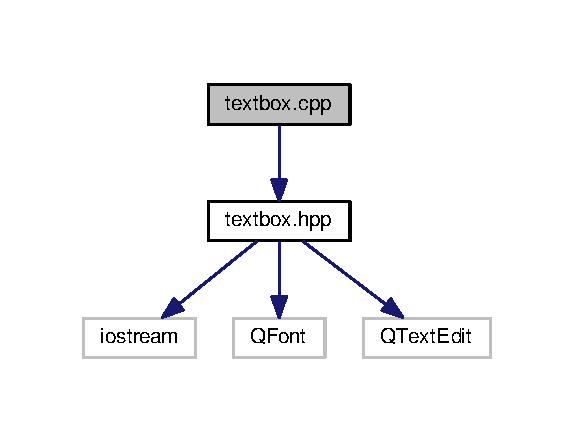
\includegraphics[width=276pt]{textbox_8cpp__incl}
\end{center}
\end{figure}


\subsection{Description détaillée}
Implementation de \hyperlink{textbox_8hpp}{textbox.\+hpp}. 



Définition dans le fichier \hyperlink{textbox_8cpp_source}{textbox.\+cpp}.


\hypertarget{textbox_8hpp}{\section{Référence du fichier textbox.\+hpp}
\label{textbox_8hpp}\index{textbox.\+hpp@{textbox.\+hpp}}
}


Gère la text box.  


{\ttfamily \#include $<$iostream$>$}\\*
{\ttfamily \#include $<$Q\+Font$>$}\\*
{\ttfamily \#include $<$Q\+Text\+Edit$>$}\\*
Graphe des dépendances par inclusion de textbox.\+hpp\+:\nopagebreak
\begin{figure}[H]
\begin{center}
\leavevmode
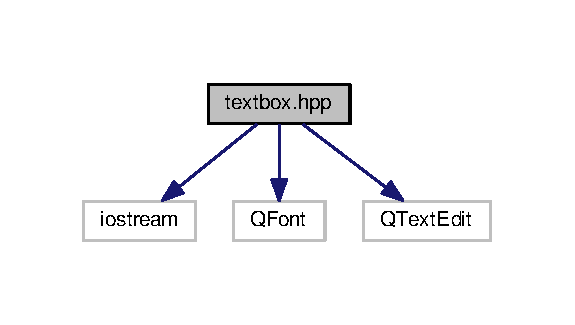
\includegraphics[width=276pt]{textbox_8hpp__incl}
\end{center}
\end{figure}
Ce graphe montre quels fichiers incluent directement ou indirectement ce fichier \+:\nopagebreak
\begin{figure}[H]
\begin{center}
\leavevmode
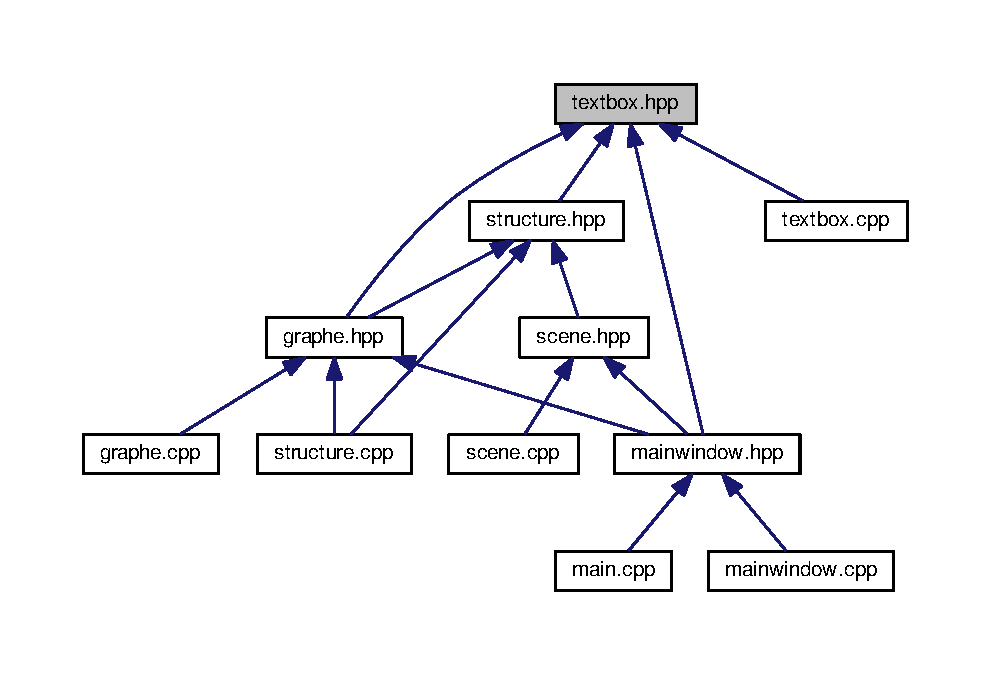
\includegraphics[width=350pt]{textbox_8hpp__dep__incl}
\end{center}
\end{figure}
\subsection*{Classes}
\begin{DoxyCompactItemize}
\item 
class \hyperlink{classTextBox}{Text\+Box}
\begin{DoxyCompactList}\small\item\em classe gerant l'affichage de texte durant l'execution \end{DoxyCompactList}\end{DoxyCompactItemize}


\subsection{Description détaillée}
Gère la text box. 



Définition dans le fichier \hyperlink{textbox_8hpp_source}{textbox.\+hpp}.


%--- End generated contents ---

% Index
\newpage
\phantomsection
\addcontentsline{toc}{chapter}{Index}
\printindex

\end{document}
